\chapter{System Design and Verification}

\section{Introduction}

The goal of this project is to determine the pose estimation error of a quadcopter in the outdoors. In this context, the pose is a six-dimensional position and orientation vector given by $P = [T | R]$, where the vector $T = [x\;y\;z]^T$ contains the translation dimensions and the matrix $R = [\theta\;\phi\;\psi]^T$ contains the roll, pitch and yaw dimensions respectively. 

In order to determine the pose estimation error of a drone, two sets of data are required, with the first being the quadcopter's own pose estimate as well as its true pose, as given by a reading from an accurate external measurement tool. There are accurate measurement tools available for the outdoor environment, which include laser and sonar systems. However, these are fairly expensive systems and the necessary equipment was not available at the time this project was executed. It was therefore decided to investigate an alternative method of measuring a quadcopter's true pose in the outdoors.

The system that was investigated, and later implemented, is a computer vision-based system. Computer vision systems (CVS) for measurement is an attractive option: they are simple, cheap, compact and easy to operate. However, the measurement accuracy of these systems differ between platforms. Therefore, a method of reliably determining a CVS's pose measurement accuracy, must also be developed before it can be used to make pose measurements.  

This chapter sets out to provide detail on the CVS.\@ First, the design and layout of the CVS is discussed. Then, the method employed to determine the pose measurement accuracy is provided, finally followed by the results of the entire process, from testing to data processing.

\section{Computer Vision System Layout}

\subsection{Introduction}

The CVS has both hardware and software components, both of which are important to making accurate measurements. In this section, the design of the CVS, including the hardware and software aspects, is discussed, providing a broad overview of what the system looks like and how it functions. 

\subsection{System Overview}

Lys requirements

The CVS is to be used to make pose measurements of a quadcopter in flight. Its measurements are to be used as accurate as possible pose data which can be used as reference pose data when comparing it to the quadcopter's on-board pose data, thereby determining the pose accuracy of a quadcopter. The CVS has to fulfil the following objectives:

\begin{itemize}
  \item Make six-dimensional pose measurements.
  \item Provide measurements with an accuracy better than the quadcopter's on-board estimate.
  \item Make reliable, consistent pose measurements.
  \item Nog?? meme
\end{itemize}

Lys metingsproses

To meet these requirements, a CVS was designed and implemented. The proposed computer vision measurement system makes use of the following processes and procedures: 

\begin{itemize}
  \item Camera calibration.
  \item Automated two-dimensional image feature extraction.
  \item Pose data extraction and derivation.
  \item Data noise elimination. 
  \item Nog?? Meme
\end{itemize}

Weet nie van hierdie deel nie...

\subsection{Software}
\label{sec:cv-sys-software}

The CVS is computer vision system, where a computer extracts information of interest from an arbitrary image. Thus, there is a string software aspect to the CVS, where the CVS relies on well-researched and understood computer vision techniques and algorithms. To this end, the open source and widely-used OpenCV library\footnote{OpenCV v2.4.8} and its sub-components was used to perform the computer vision tasks. This library was used since its free, readily available, has a wide support network on the internet and come pre-packaged with a large variety of up-to-date and powerful computer vision functions. To perform the numerical operations, the open-source NumPy\footnote{NumPy v1.8.2} library was used. 

The OpenCV library was used to extract feature data from a video stream, calibrate the CVS's camera and determine the pose of a calibration pattern by solving the principle n-points (PnP) problem. The entire process takes place as follows. 

First, the camera is calibrated by following the procedure discussed in Chapter meme. Here, a $5\times6$ square chessboard pattern was used for calibration. To summarise the procedure, the OpenCV functions `findChessboardCorners()' and `findConrersSubPix()' are used to detect and extract two-dimensional coordinate data of the corners on the chessboard pattern from a still image. These coordinates, along with their three-dimensional world coordinates, are fed to the `calibrateCamera()' function to produce the camera matrix. The calibration procedure produced the camera matrix $C$, as presented in Equation~\ref{eq:chap2-cam-matrix} and repeated again in Equation~\ref{eq:chap3-cam-matrix} for convenience. 

\begin{equation}
  \label{eq:chap3-cam-matrix}
  C = 
  NP
\end{equation}

In Equation~\ref{eq:chap3-cam-matrix}, the matrix $N$ is given by Equation~\ref{eq:chap3-cam-intrinsic} and matrix $P$ by Equation~\ref{eq:chap3-cam-extrinsic}.

\begin{equation}
  \label{eq:chap3-cam-intrinsic}
  N = 
  \begin{bmatrix}
    f_x & 0   & u_0 \\
    0   & f_y & v_0 \\
    0   & 0   & 1   \\
  \end{bmatrix}
\end{equation}

\begin{equation}
  \label{eq:chap3-cam-extrinsic}
  P = 
  \begin{bmatrix}
    R | T
  \end{bmatrix}
  =
  \begin{bmatrix}
    r_{11} & r_{21} & r_{31} & t_1 \\
    r_{21} & r_{22} & r_{32} & t_2 \\
    r_{31} & r_{23} & r_{33} & t_3 \\
  \end{bmatrix}
\end{equation}

With the calibrated camera matrices, $N$ and $P$, it is now possible to perform camera pose estimation. This procedure is based on the relation given in Equation~\ref{eq:chap3-2d-to-3d}, which relates the three-dimensional world coordinate system $X_w$ to its two-dimensional image projection $x_c$.  

\begin{equation}
   \label{eq:chap3-2d-to-3d}
   x_c
   = C
   X_w
\end{equation}

Using the relation in Equation~\ref{eq:chap3-2d-to-3d} and the camera matrix $C$'s intrinsic parameters, OpenCV's `solvePnPRansac()' function can be employed to extract the pose matrix $P$ of the camera relative to the calibration board. The PnP solver used is the robust PnP solver, employing Leverberg-Marquart optimsisation, as described by~\cite{schweighofer2006robust}. It was found that a $5\times6$ chessboard does not have enough features to guaruntee accurate results from the ePnP method of~\cite{lepetit2009epnp}.

\subsection{Hardware}

The hardware requirements for the CVS are minimal and its setup is very simple. To perform six-dimensional pose estimations, the hardware only needs to capture image data at a high enough frame rate and resolution for the OpenCV algorithms to be able to detect and extract feature information. A computer for data processing tasks, as well as a calibration board, is also required. 

To meet these requirements, a single camera can be used to capture still or video image data, along with a chessboard calibration pattern and laptop running the pose estimation software.  

A stereo camera setup can also be used, however, the accuracy between the single and stereo camera in most respects is rather negligible, except in the depth dimension where the stereo vastly outperforms the single camera. This is to be expected and is very akin to a person's depth perception abilities being compromised with one eye closed. For this implementation, the single camera variant was selected. This makes the system simpler to set up and use. However, care must be taken with the depth estimation when using a single camera. In the future, the project can be expanded to a stereo camera system if it is found that the inaccurate depth estimate compromises the measurement accuracy.

For the pose estimation software to work best, it requires a clear view of the calibration pattern. Therefore, a big calibration pattern is desirable. Furthermore, the pattern should of a high quality and printed on white paper with a wide white border to enhance the contrast between the pattern and the background, making it easier for the software to detect the pattern. 

\section{Measurement Test Design}

\subsection{Introduction}

Before the CVS was used to record the pose data of a drone, the accuracy of the system's measurements was first determined. Since the PnP solving algorithm is, at its core, an optimisation problem and produces estimates of the pose, determining the accuracy of the CVS is an important step in the system design phase. 

To determine the measurement error, a measurement test was performed in an indoor environment where an external measurement device recorded pose data. The error was then be determined by comparing the CVS's measurements with that of the external measurement system's measurement data. Both systems were set to record the pose of a flat chessboard calibration pattern that was moved and orientated by hand.

This section describes the test layout, including the external measurement device and its details, as well as the CVS's details. Then, the measurement procedure is presented, followed by the steps taken to process the data during the post-processing phase. 

\subsection{Test Layout}
\label{sec:vicon-test-setup}

\subsubsection{External Measurement Device Layout}

The external measurement system used to record the ground-truth data that was used to compare the CVS's measurements to, is a Vicon indoor motion capture system. It is a widely-used commercial system with applications in the film, medical and sporting industries and can reach sub-millimetre accuracy in its measurements. It works by tracking a set of infrared markers stuck to a surface, with at least two infrared cameras and sophisticated proprietary motion tracking software. It does this at a rate of 300Hz, or 300 FPS.\@ Given its accuracy, the measurement results from this system was taken as ground-truth.

The Vicon system used for the test is located in the 3D Human Motion Laboratory on Stellenbosch University's Tygerberg medical campus. It consists of eight infrared cameras arranged around a square on the floor in a configuration that maximises the number of infrared markers visible to each camera at any given point in time. Figure~\ref{fig:chap3-vicon-layout} shows a diagram of the Vicon system layout. 
 
\begin{figure}
  \centering
  \def\svgwidth{0.5\textwidth}
  \input{figures/chapter3/vicon_layout.pdf_tex}
  \caption[Layout of the Vicon motion capture system.]{Layout of the Vicon motion capture system. Note that this is not drawn to scale.}
\label{fig:chap3-vicon-layout}
\end{figure}

Before the test commenced, the Vicon system was calibrated and the infrared markers were placed on both the calibration board and camera frame used by the CVS\@. Since the Vicon and CVS camera each have their own coordinate systems, having the position and orientation of the CVS camera available will allow the Vicon's measurements to be related back to the CVS's camera coordinate system during the data processing phase. The markers were placed in such a way that they will produce axes that more or less coincides with the Vicon's axis system, slightly reducing the work load during the data processing phase. Figure~\ref{fig:chap3-cam-vicon-axes} shows the axis system's for both the CVS and Vicon systems.

\begin{figure}
  \centering
  \def\svgwidth{0.5\textwidth}
  \input{figures/chapter3/cam_vicon_axis.pdf_tex}
  \caption{The axis orientations of the Vicon and CV systems.}
\label{fig:chap3-cam-vicon-axes}
\end{figure}

Only three markers are required to be visible for the Vicon system to produce a six-dimensional pose vector, but a fourth asymmetrical auxiliary marker was placed to provide fail-safe orientation data during the post-processing phase. Figures~\ref{fig:chap3-cam-marker-placement} and~\ref{fig:chap3-board-marker-placement} show the marker placements for the camera and the calibration board. These markers were carefully placed by hand, but there will be some placement error nonetheless. This error offset is taken into account during the data processing phase. 

\begin{figure}
   \centering 
   \includegraphics[clip, trim = 0 400 0 400, width=0.6\textwidth]{figures/chapter3/cam_1.pdf}
   \caption{Infrared marker placement on the camera.}
\label{fig:chap3-cam-marker-placement}
\end{figure}

\begin{figure}
   \centering 
   \includegraphics[clip, trim = 600 0 400 0, width=0.6\textwidth]{figures/chapter3/bord_2.pdf}
   \caption{Infrared marker placement on the chessboard.}
\label{fig:chap3-board-marker-placement}
\end{figure}

One aspect of the Vicon system to note is that the infrared markers have some high-frequency noise associated with them, which is apparent when inspecting the raw data. This noise is inherent to the marker and can be safely filtered out with a zero-lag, second order Butterworth filter. However, the raw, unfiltered data is used throughout this project. 

\subsubsection{Computer Vision System Setup}

The CVS consists out of a single Microsoft LifeCamHD webcam, capable of recording 720p High-Definition (HD) video data at 30 frames per second (FPS), an A1, $5\times6$ square chessboard pattern, generated by OpenCV's pattern generator, and a laptop running the image capturing and processing software. The webcam's focus, image resolution, FPS rate and exposure was controlled from the laptop using he `uvcdynctrl' script from the libwebcam library\footnote{uvcdynctrl v0.2.4, bit.ly/1E4ARv3}. 

Before the test, the camera was calibrated to determine its camera matrix and focal lengths in the $x$ and $y$ directions. Calibration was done with the same board and camera that was used during the test, against a white, well-lit background. The board was moved to different positions and orientations within view of the camera, and roughly 15 still images in standard resolution ($640\times480$ pixels) were taken. The camera was then calibrated with this set of images and OpenCV's camera calibration module to produce a camera matrix that gives a reprojection error of between 0.18 and 0.21 pixels. It was found that capturing data at a higher resolution did not produce significantly better results and slowed the data extraction process down. 

In the test, the camera was placed in a stable aluminium frame and was left untouched throughout the test. The laptop was set to only capture video at $640\times480$ pixels, while zoom and autofocus was disabled to keep the camera's lens focus constant to the focal length that was found during calibration. The focal length was found to be approximately 700 pixel units in both the $x$ and $y$ direction. The data extraction and pose estimation took place off-line. 

\subsection{Test Procedure}

Figure~\ref{fig:chap3-pic-sys-layout} shows a picture of the complete test setup. As described in Section~\ref{sec:vicon-test-setup}, the camera is placed on a chair and the board is held facing the camera. Both of these are covered with four infrared markers with the eight infrared cameras surrounding both the board and camera.  

\begin{figure}
  \centering
  \includegraphics[clip, trim = 600 300 0 0, width=0.7\textwidth]{figures/chapter3/sys_1.pdf}
  \caption{Picture of the test layout.}
\label{fig:chap3-pic-sys-layout}
\end{figure}

Data capture started when the Vicon system started recording. At the same time, the chessboard was tilted forward. This allowed for both measurement data sets to be synchronised to a common timeframe during the data processing phase. During the data capturing phase, the board was moved by hand to different positions and orientations with respect to the CVS's camera axis system to generate measurement data vectors with both the CVS and Vicon. To produce a diverse cloud of data vectors, the board was moved around the full field of view and at different distances to the camera, while simultaneously varying the board's rotation angles. Each video is approximately 90 seconds long, which equates to close to 2700 pose vector samples per test, though it was decided that only 2400 of these points will be used to compensate for any invalid or inconsistent readings. 

The test produced two sets of measurement data: one ground-truth pose measurement data set from the Vicon system, and one data set from the CVS\@. These data sets allows for the determination of the CVS's measurement error by comparing the two sets of measurement. These sets were also used to provide training and validation data sets for a error prediction model, which is discussed in Chapter MEMEMEMEME.\@

\subsection{Data Processing}

\subsubsection{Introduction}

During the test, the CVS only captured video data, leaving the data extraction and pose estimation to be done off-line during the data processing phase. The Vicon system data requires very little processing, since most of the data is generated in real-time and is optimised by the Vicon software. However, some work was done to fix invalid measurements that were introduced when not enough Vicon cameras had a good view of the infrared markers for a few frames. These points were corrected by means of interpolation. Furthermore, because the Vicon is a stationary system, it was convenient to move and rotate the CVS's camera and chessboard pose data to coincide with the Vicon's axis system.

Processing the CVS data involves several steps, which include simultaneously optimising the camera's focal length and the infrared marker offsets and then determining the accuracy of the CVS pose estimation system. Each of these aspects are discussed next.

\subsubsection{Rotating the Camera and Chessboard Data}
\label{sec:rotate-axes}

During the test, four markers were placed on the CVS camera frame to provide data on its placement. These markers were placed along the camera's $x$ and $y$ axes and coincides with the chessboard's axis system. 

With the CVS's camera placement and orientation in the Vicon coordinate system known, relocating and reorientating the CVS's camera pose data to coincide with the Vicon's axis system becomes a simple task. The CVS's pose within the Vicon system is constant and the CVS's measurements are made relative to its camera's axis system. Therefore, relocating and reorientating the chessboard's pose data to coincide with the Vicon's axis system was done by simply subtracting the CVS's camera placement pose from each pose vector of the chessboard.

With the CVS's camera axis system now centred around the Vicon system's origin, the pose data for the chessboard acquired by the CVS and the Vicon are directly relatable. 

\subsubsection{Camera Parameter Optimisation}
\label{sec:focal-optimisation}

Before the test took place, the CVS camera was calibrated using OpenCV's camera calibration toolbox. This procedure provides a fairly good estimate of the intrinsic parameters of the camera, which includes the focal lengths. However, given the lack of reference three-dimensional data, it is only an estimate. Using the ground-truth Vicon pose data will allow the focal length to be determined more accurately. At the same time, the distance offset between the true infrared marker centre and the ideal infrared marker centre also needs to be taken into account. This offset will also account for any constant measurement bias introduced by the CVS\@. This presents a circular optimisation problem: the focal length will affect the perceived offset, while the offset will affect the CVS pose estimates, which in turn affects the ideal focal length. To find the offset and optimum focal length, a dual optimisation strategy was implemented.  

First, the optimisation algorithm is formulated. Suppose $\bm{P}^*$ denotes the six-dimensional pose vector as given by the Vicon system, while $\bar{\bm{P}}$ is the constant offset vector and the subscripts $c$ and $b$ represent the camera and board respectively. $\bm{\epsilon}$ is the error between the Vicon and CVSs' measurements that needs to be determined and $\bm{F}(f)$ is the pose vector measured by the CVS's camera, as a function of its focal lengths $f_x$ and $f_y$. The Vicon pose and offset vectors are then given by the Equations~\ref{eq:chap3-pose} and~\ref{eq:chap3-offset}.

\begin{equation}
 \label{eq:chap3-pose}
  \bm{P}^* = \bm{P}^*_b - \bm{P}^*_c
\end{equation}

\begin{equation}
  \label{eq:chap3-offset}
  \bar{\bm{P}} = \bar{\bm{P}}_b - \bar{\bm{P}}_c
\end{equation}

The equation for the pose estimate given by the CVS is given by Equation~\ref{eq:chap3-cvs}.

\begin{equation}
  \label{eq:chap3-cvs}
  \bm{F}(f) = \bm{P}^* - \bar{\bm{P}} + \bm{\epsilon}
\end{equation}

Equation~\ref{eq:chap3-cvs} can then be simplified to the form given in Equation~\ref{eq:chap3-pose}, which forms the basis of the optimisation algorithm. 

\begin{equation}
  \label{eq:chap3-pose}
  \bm{F}(f_x, f_y) = (\bm{P}^*_b - \bar{\bm{P}}_b) - (\bm{P}^*_c - \bar{\bm{P}}_c) + \bm{\epsilon}
\end{equation}

The next step is to determine the constant perceived offset for a given focal length. The focal length is initialised with the focal length given by the calibration procedure (approximately 700 pixel units). The offset is then determined by using Equation~\ref{eq:chap3-eq1-offset}.

\begin{equation}
  \label{eq:chap3-eq1-offset}
  \sum\limits_i \bm{F}_i(f) - \sum\limits_i(\bm{P}^*_{b,i} - \bm{P}^*_{c, i}) = i\bar{\bm{P}} + \sum\limits_i\bm{\epsilon}_i
\end{equation}

At this point, it is assumed that the error vector $\bm{\epsilon}$ is normally distributed around $0$, thereby eliminating it's sum and leading to Equation~\ref{eq:chap3-eq2-offset}. This assumption will be verified in Section~\ref{sec:err-norm-test}. 

\begin{equation}
  \label{eq:chap3-eq2-offset}
  i\bar{\bm{P}} = \sum\limits_i \bm{F}_i(f) - \sum\limits_i(\bm{P}^*_{b,i} - \bm{P}^*_{c, i})
\end{equation}

Using the constant $\bar{\bm{P}}$ produced by Equation~\ref{eq:chap3-eq2-offset}, it is now possible to minimise the error $\bm{\epsilon}$ from Equation~\ref{eq:chap3-pose} by varying the focal lengths, $f_x$ and $f_y$. The minimum focal lengths were found by first setting up a $3\times n$ error matrix, consisting of the three translation dimensions, ${[x\;y\;z]}^T$, where $n$ is the number of samples in the data set. The optimisation is based on these three dimensions, since it was found that including the rotation dimensions added too much variability to the procedure, leading to instability. The error matrix is produced by Equation~\ref{eq:chap3-error-base}.

\begin{equation}
  \label{eq:chap3-error-base}
  \bm{\epsilon} = \bm{F}(f) - \bm{P}^* - \bar{\bm{P}}
\end{equation}

Using the $3\times n$ error matrix found in Equation~\ref{eq:chap3-error-base}, an error vector is generated by summing the matrix along its columns. The optimum focal lengths are then found by taking the focal length combination that produces the smallest 2-norm of the error vector $\bm{\epsilon}$. The equation is given by Equation~\ref{eq:chap3-err-min}.

\begin{equation}
  \label{eq:chap3-err-min}
  \min_{f_x, f_y}\left \Vert \sum_i  \bm{\epsilon}_i \right \Vert
\end{equation}

With the optimal focal length now determined, the process starts again from Equation~\ref{eq:chap3-pose}, finding a new offset for the new focal length. This procedure is iterated a set number of times, minimising the total error norm. After the optimum focal length combination was found, that combination was used in the camera matrix that extracted the pose data from the video data.

In summation, the algorithm is as follows:

\begin{enumerate}
  \item Initialise focal lengths with values from the calibration procedure. 
  \item Repeat $k$ times:
  \begin{enumerate}
    \item Find $\bar{\bm{P}}$ for a constant $f_x$ and $f_y$ (Equation~\ref{eq:chap3-offset}).
    \item Determine the error vector $\bm{\epsilon}$ with new $\bar{\bm{P}}$ (Equation~\ref{eq:chap3-error-base}).
    \item Update focal lengths $f_x$ and $f_y$ with focal length that minimises $\left \Vert \bm{\epsilon} \right \Vert$ (Equation~\ref{eq:chap3-err-min}).
  \end{enumerate}
  \item Use new focal lengths to estimate the chessboard's pose.
\end{enumerate}

\section{Results}

\subsection{Introduction}

During the optimisation procedure, it was assumed that $\bm{\epsilon}$ was normally distributed around 0. In this section, it is proven that this is indeed the case. Convergence of the optimisation procedure is also proven, and the results of the CVS's pose estimates, and its measurement error, are presented and discussed.

\subsection{Proof of Convergence}

To test for convergence, the total error for each dimension after an entire iteration of the optimisation was determined and plotted. Figure~\ref{fig:err-convergence} shows the errors of the $\bm{\epsilon}$ vector over 50 iterations.

\begin{figure*}
  \centering
  \begin{subfigure}{0.45\textwidth}
    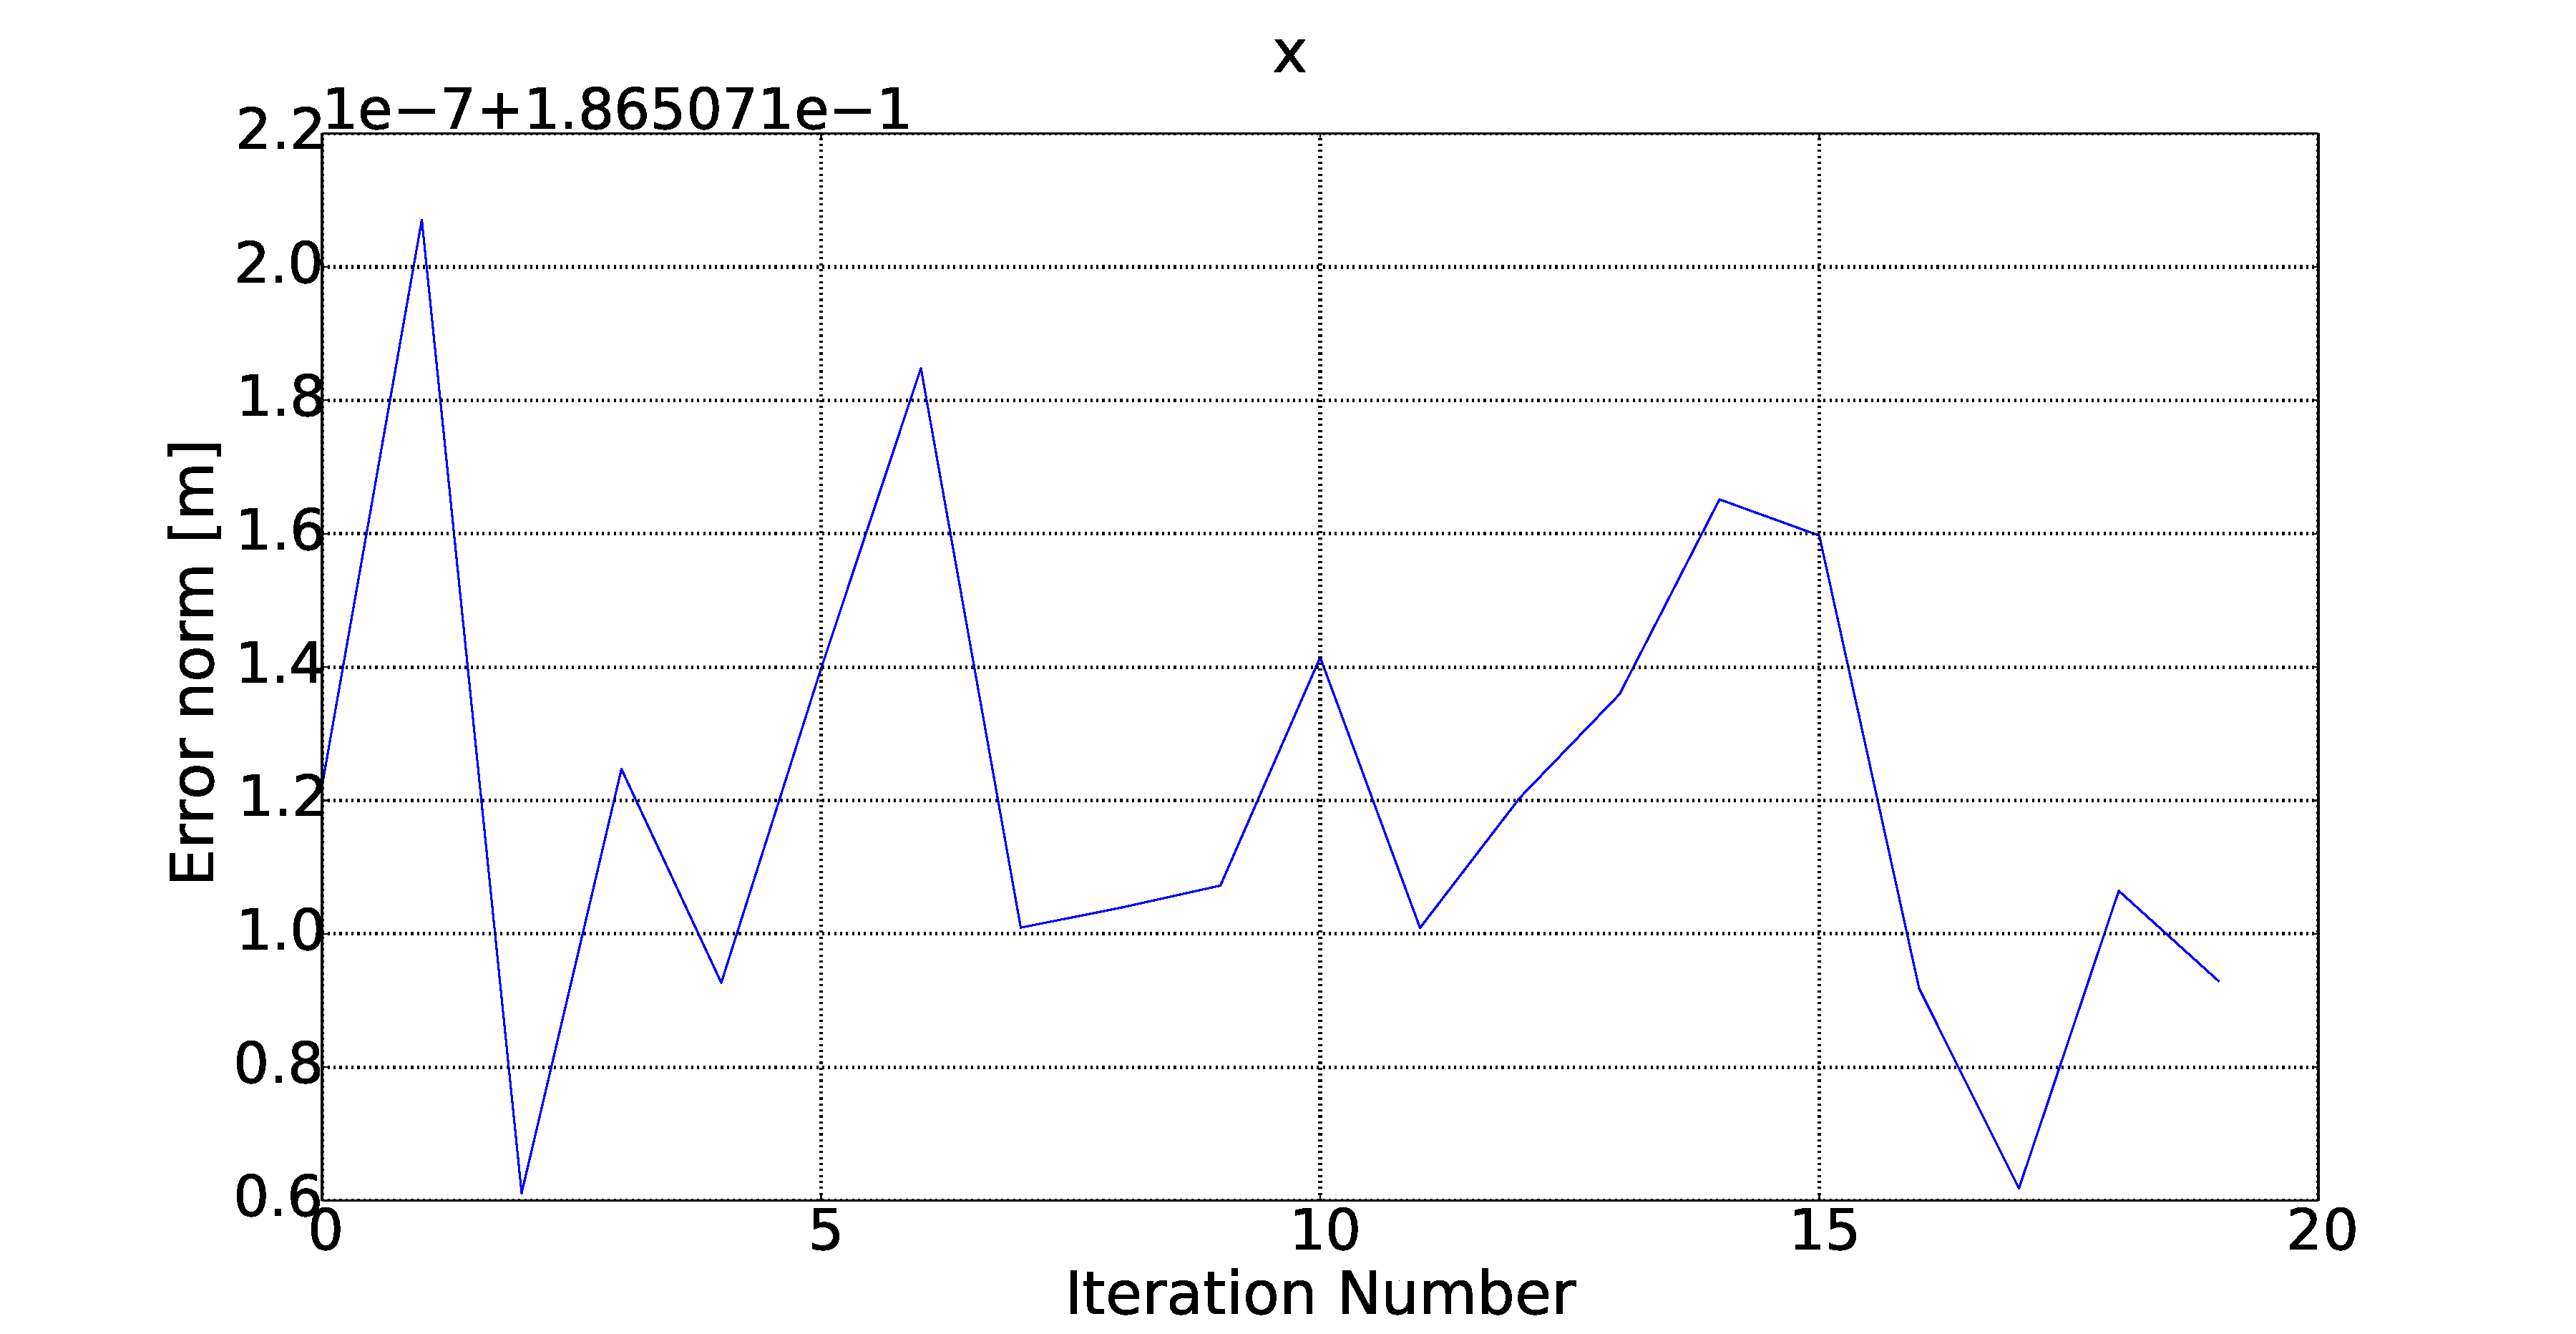
\includegraphics[width=\textwidth]{figures/chapter3/err_x.pdf}
    \caption{Error convergence in the $x$ dimension [m].}
\label{fig:err-convergence-x}
  \end{subfigure}
~
  \begin{subfigure}{0.45\textwidth}
    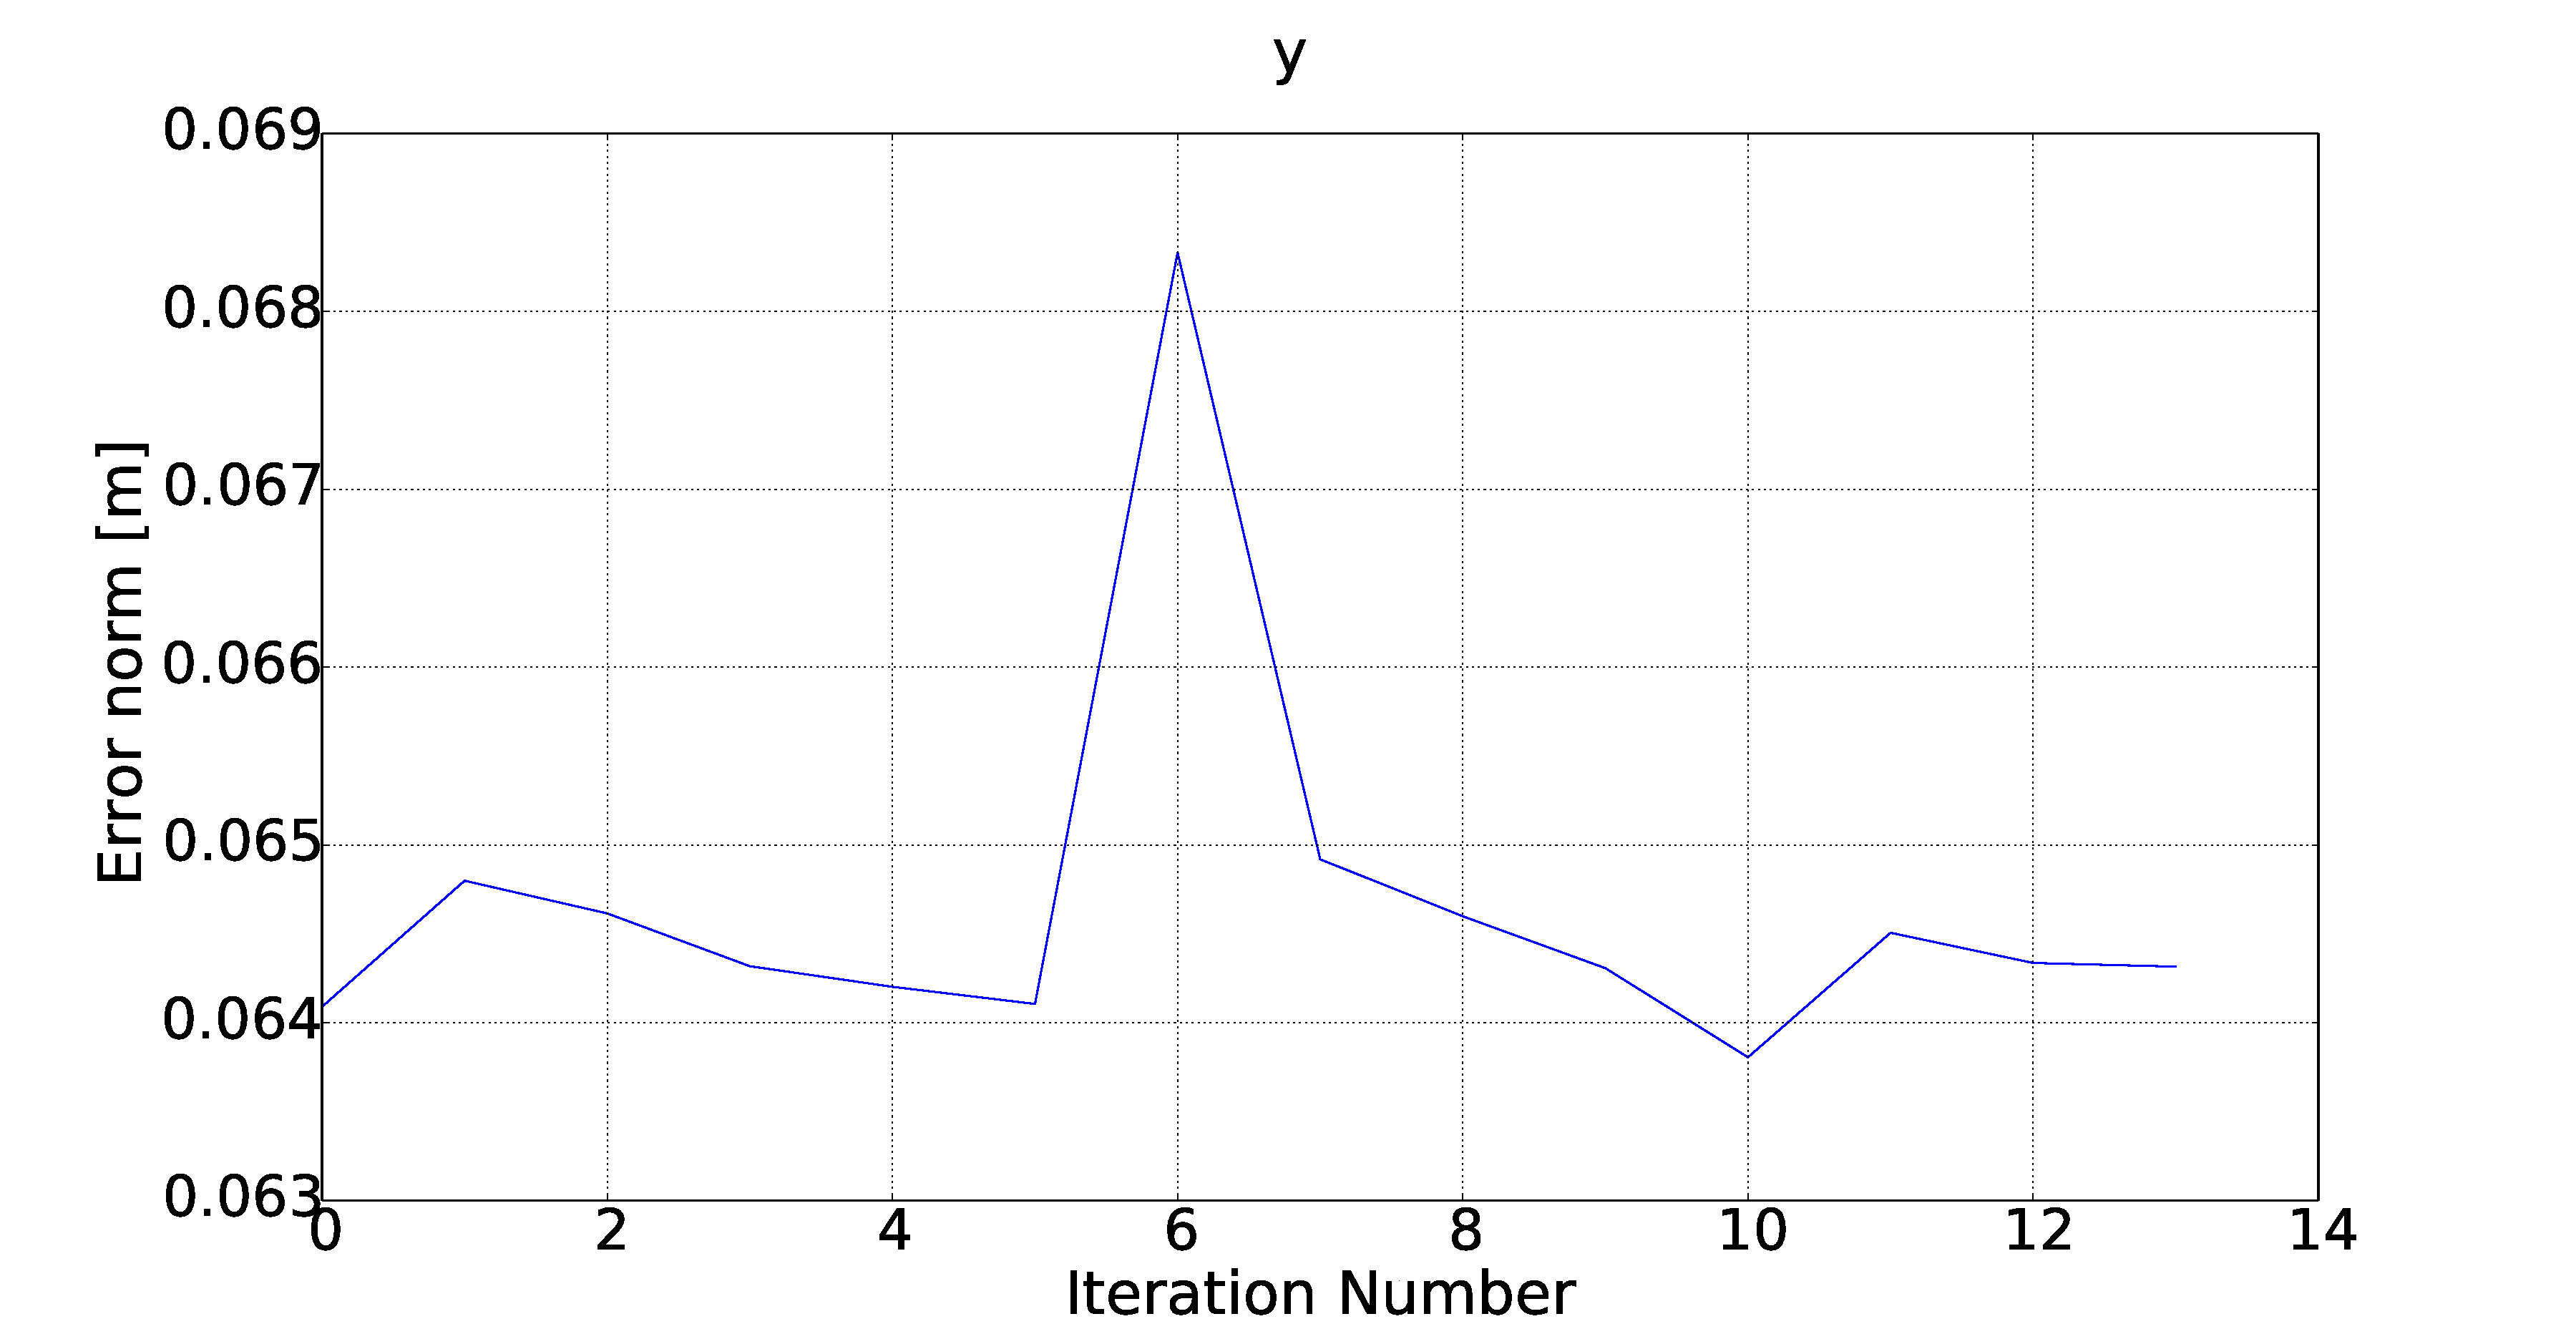
\includegraphics[width=\textwidth]{figures/chapter3/err_y.pdf}
    \caption{Error convergence in the $y$ dimension [m].}
\label{fig:err-convergence-y}
  \end{subfigure}
~
\begin{subfigure}{0.45\textwidth}
    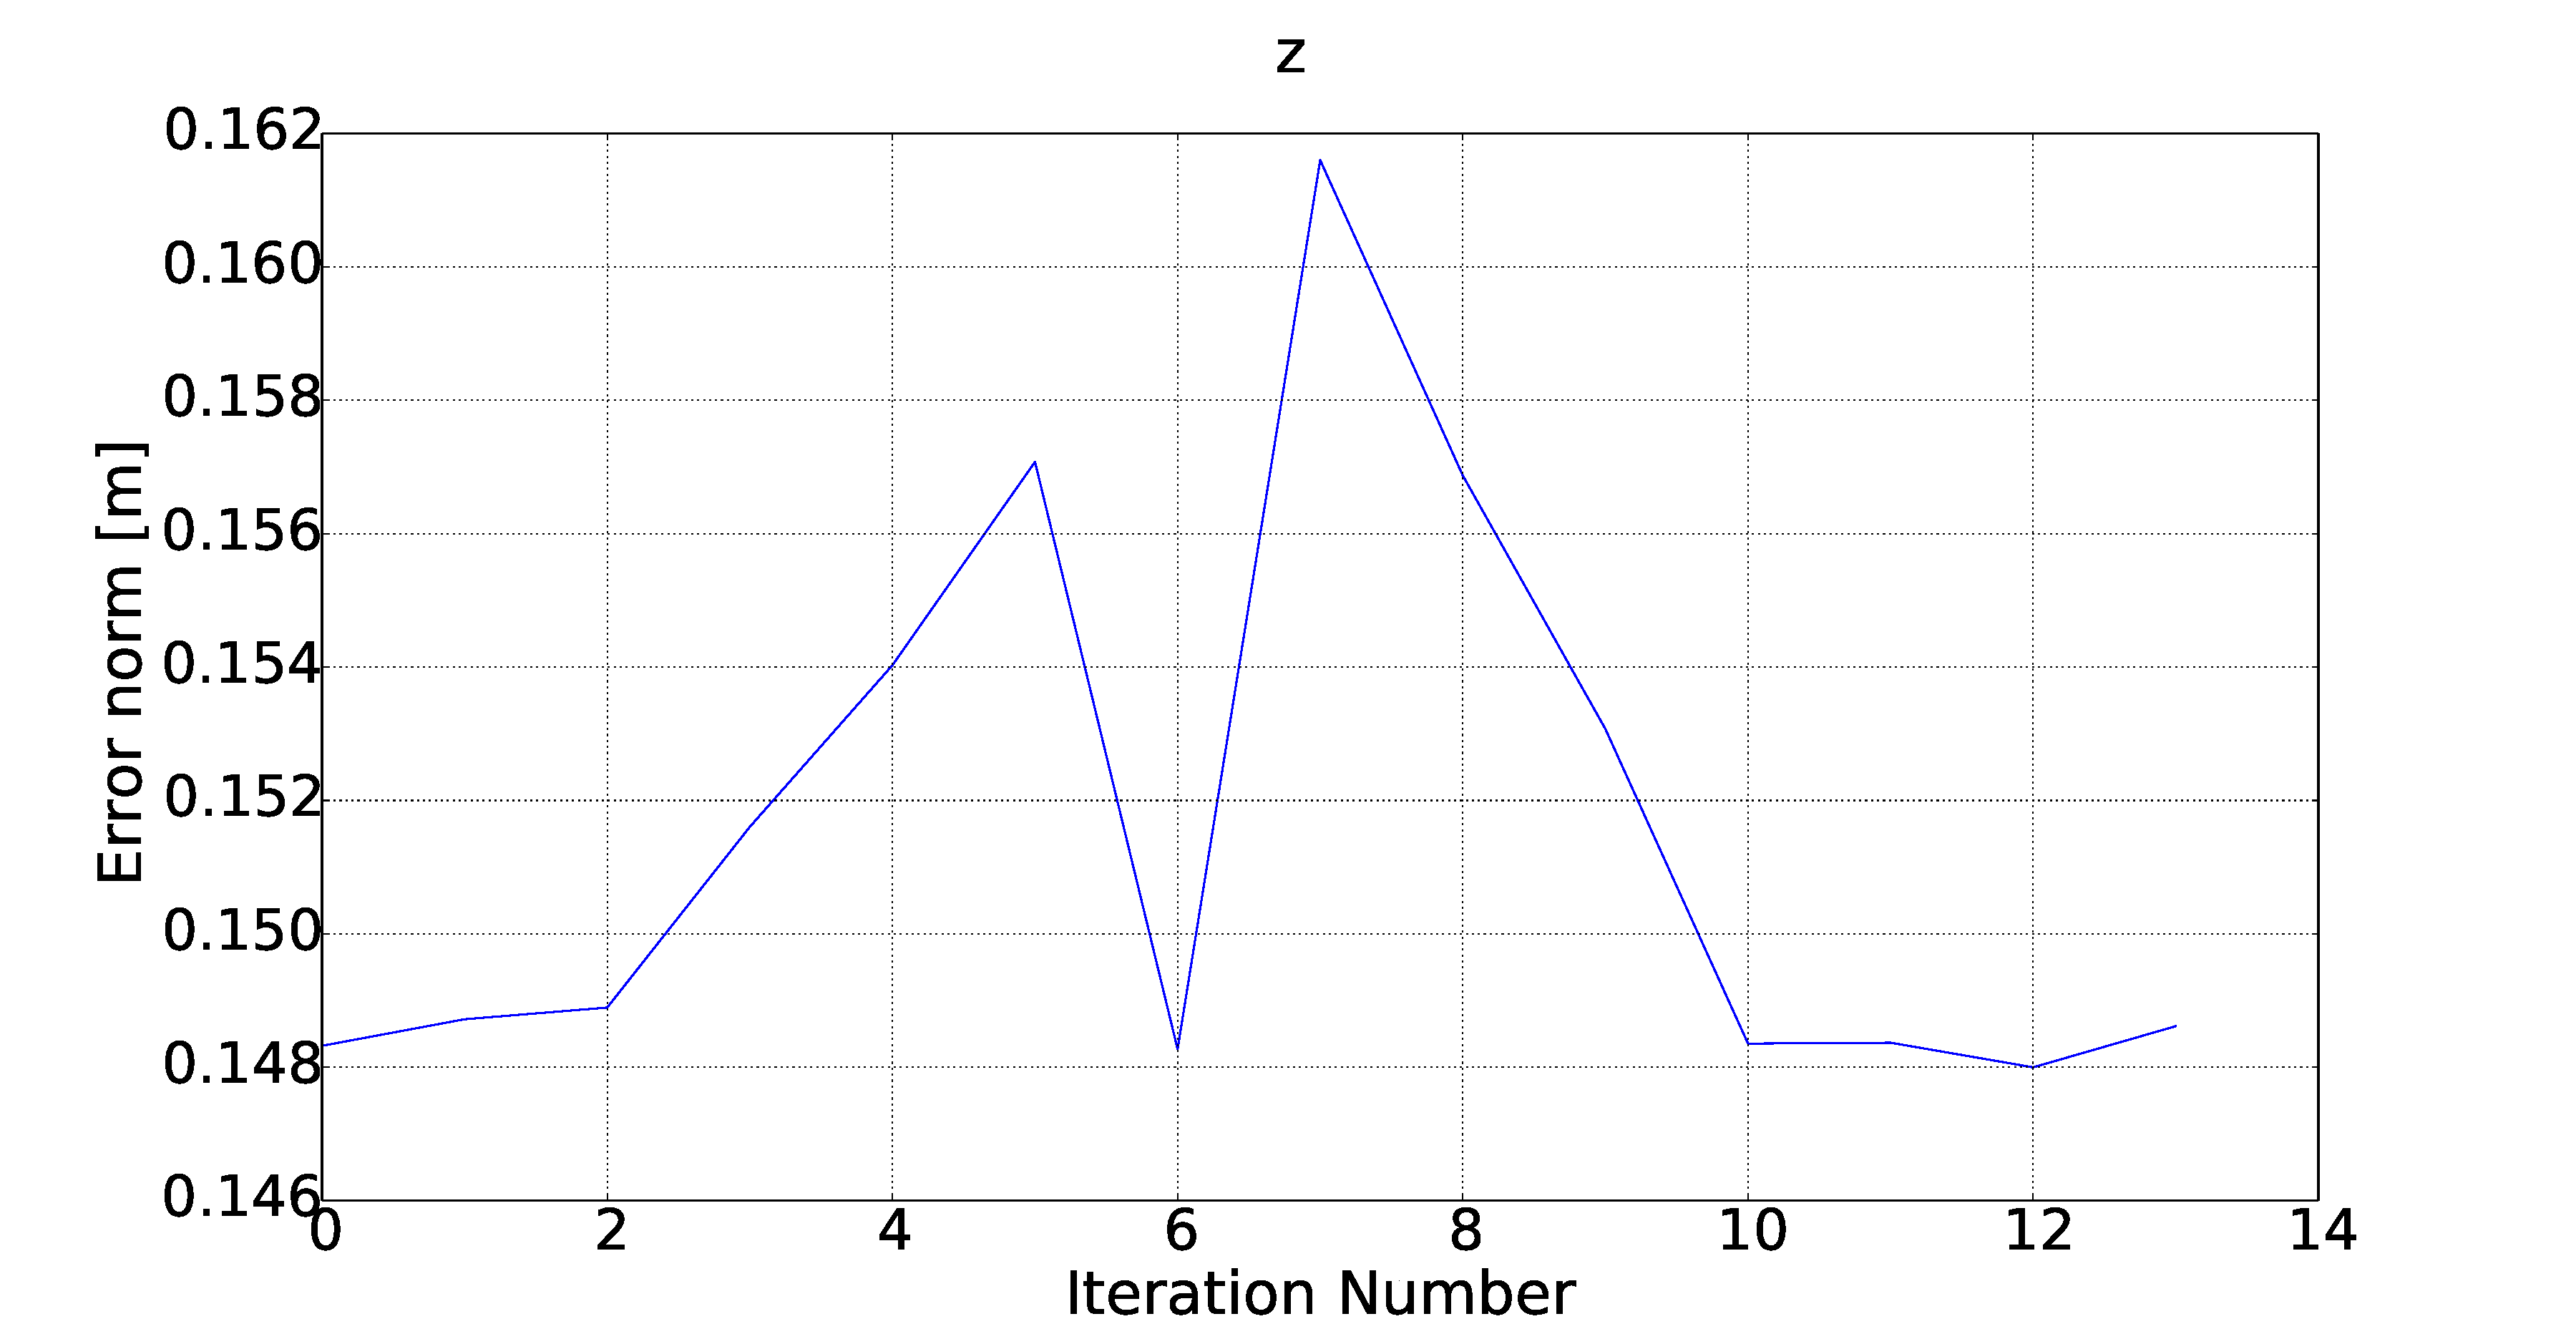
\includegraphics[width=\textwidth]{figures/chapter3/err_z.pdf}
    \caption{Error convergence in the $z$ dimension [m].}
\label{fig:err-convergence-z}
  \end{subfigure}
~
  \begin{subfigure}{0.45\textwidth}
    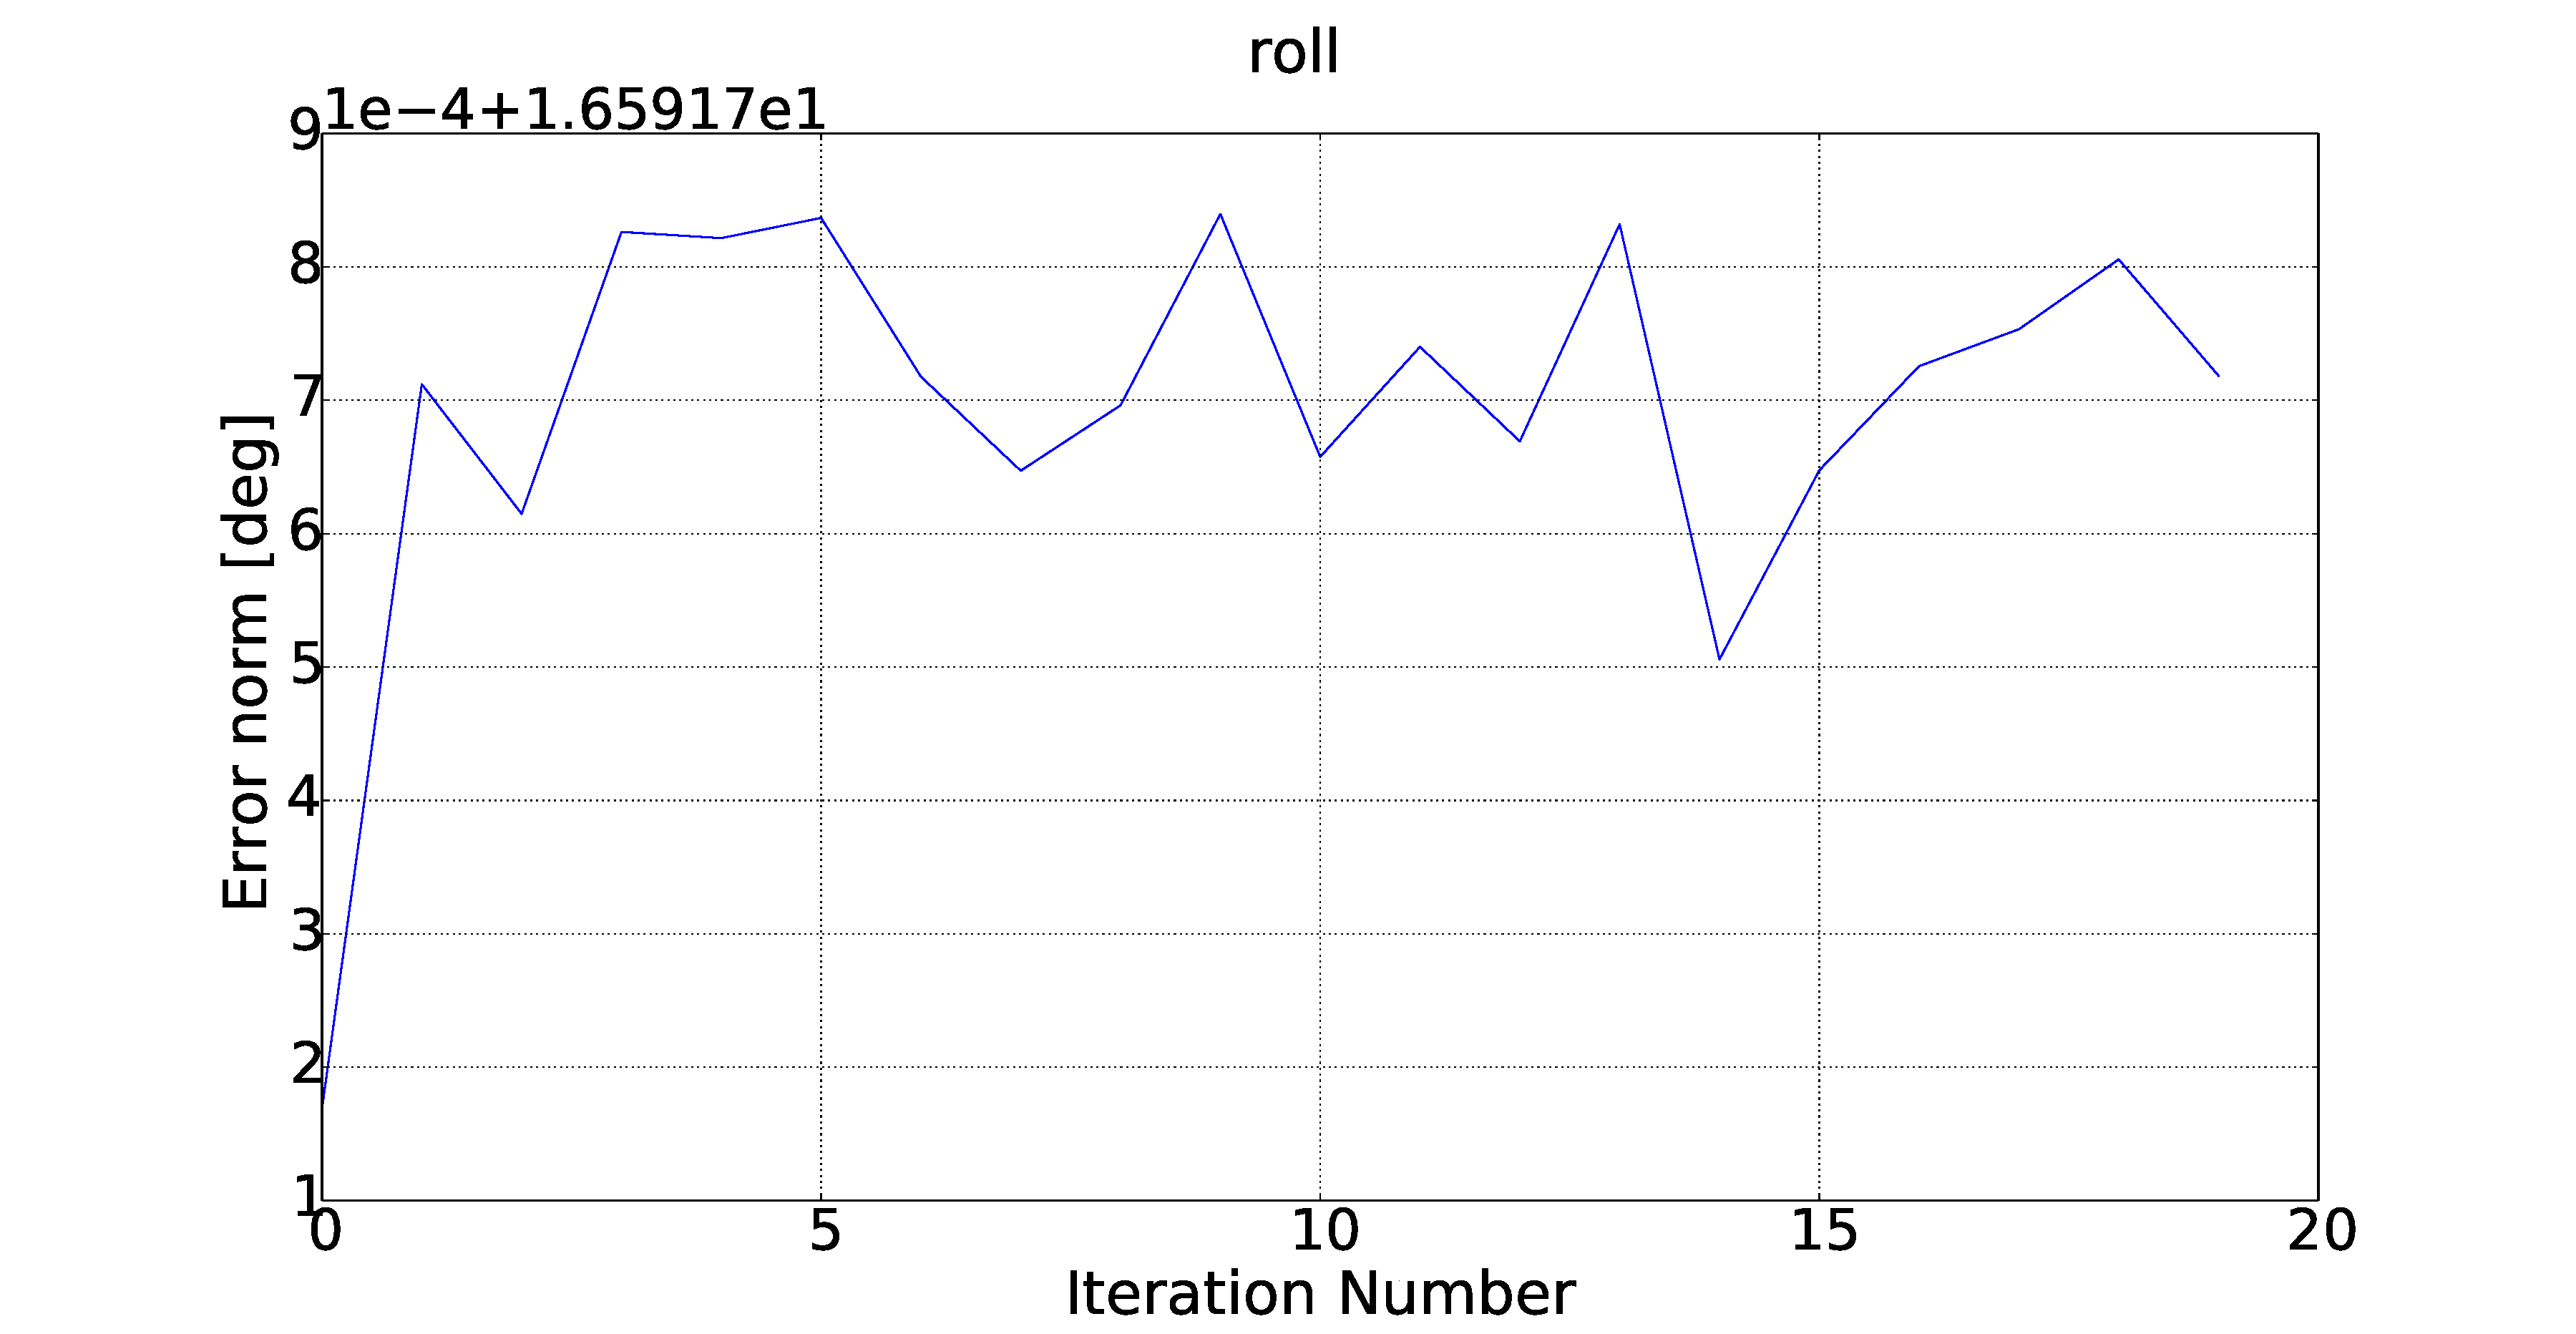
\includegraphics[width=\textwidth]{figures/chapter3/err_roll.pdf}
    \caption{Error convergence in the $\theta$ dimension [degrees].}
\label{fig:err-convergence-roll}
  \end{subfigure}
~
  \begin{subfigure}{0.45\textwidth}
    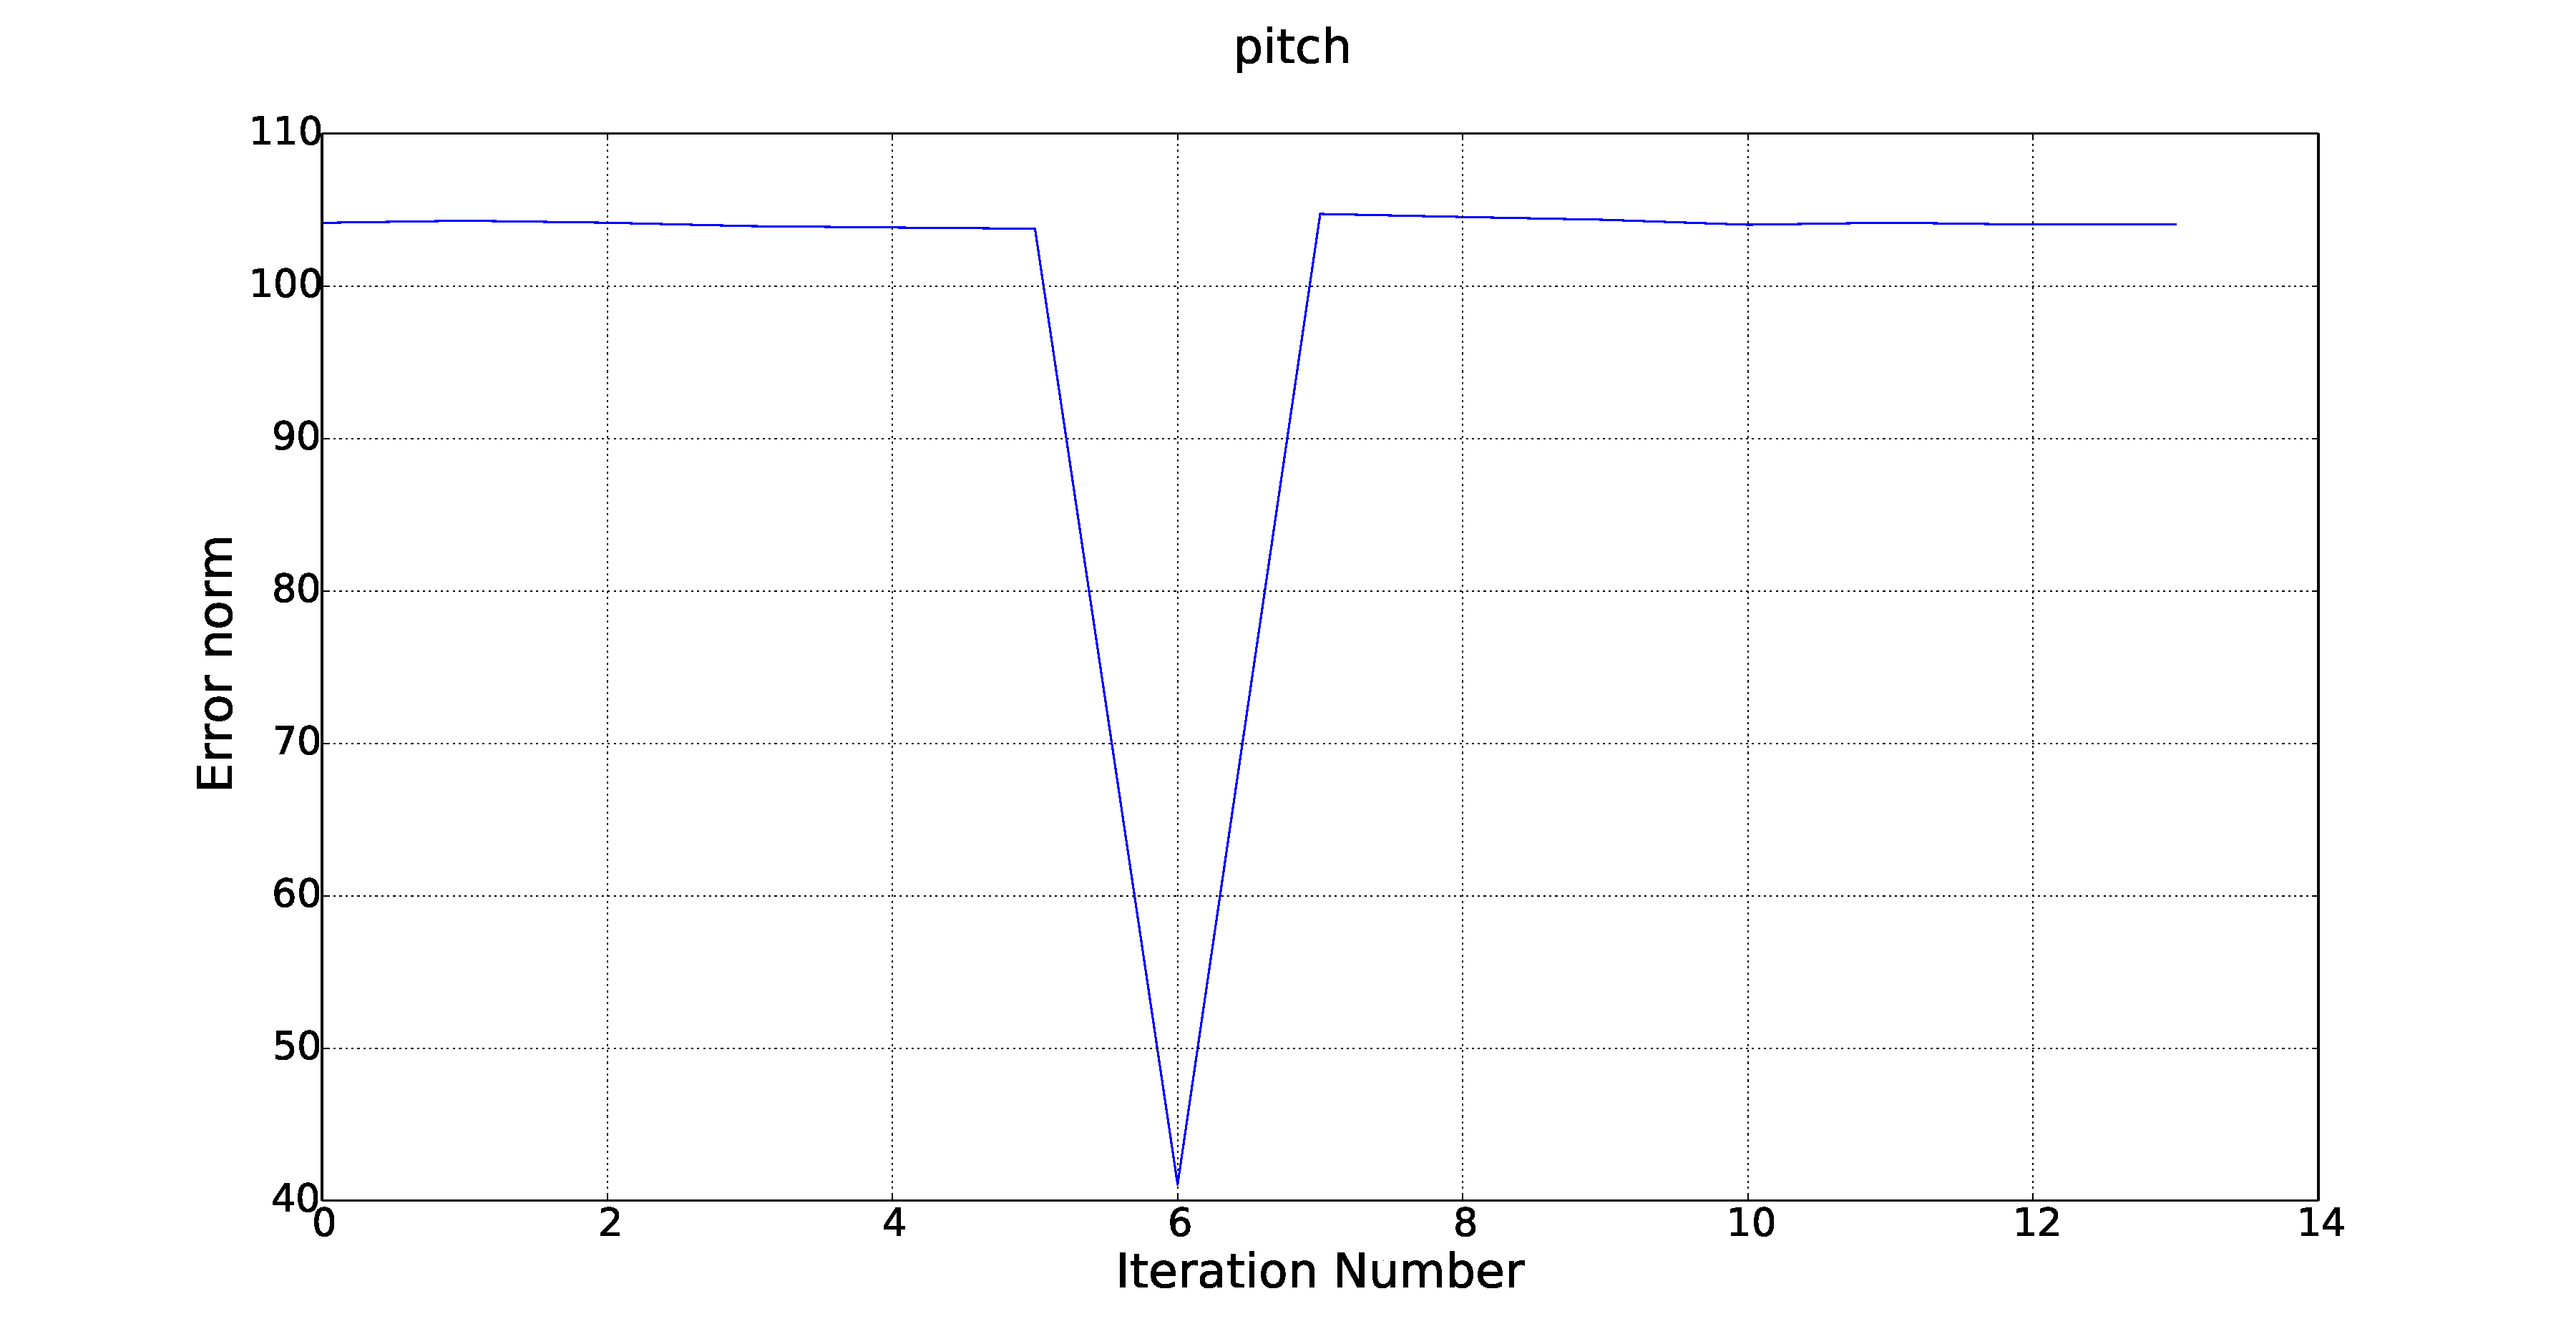
\includegraphics[width=\textwidth]{figures/chapter3/err_pitch.pdf}
    \caption{Error convergence in the $\phi$ dimension [degrees].}
\label{fig:err-convergence-pitch}
  \end{subfigure}
~
  \begin{subfigure}{0.45\textwidth}
    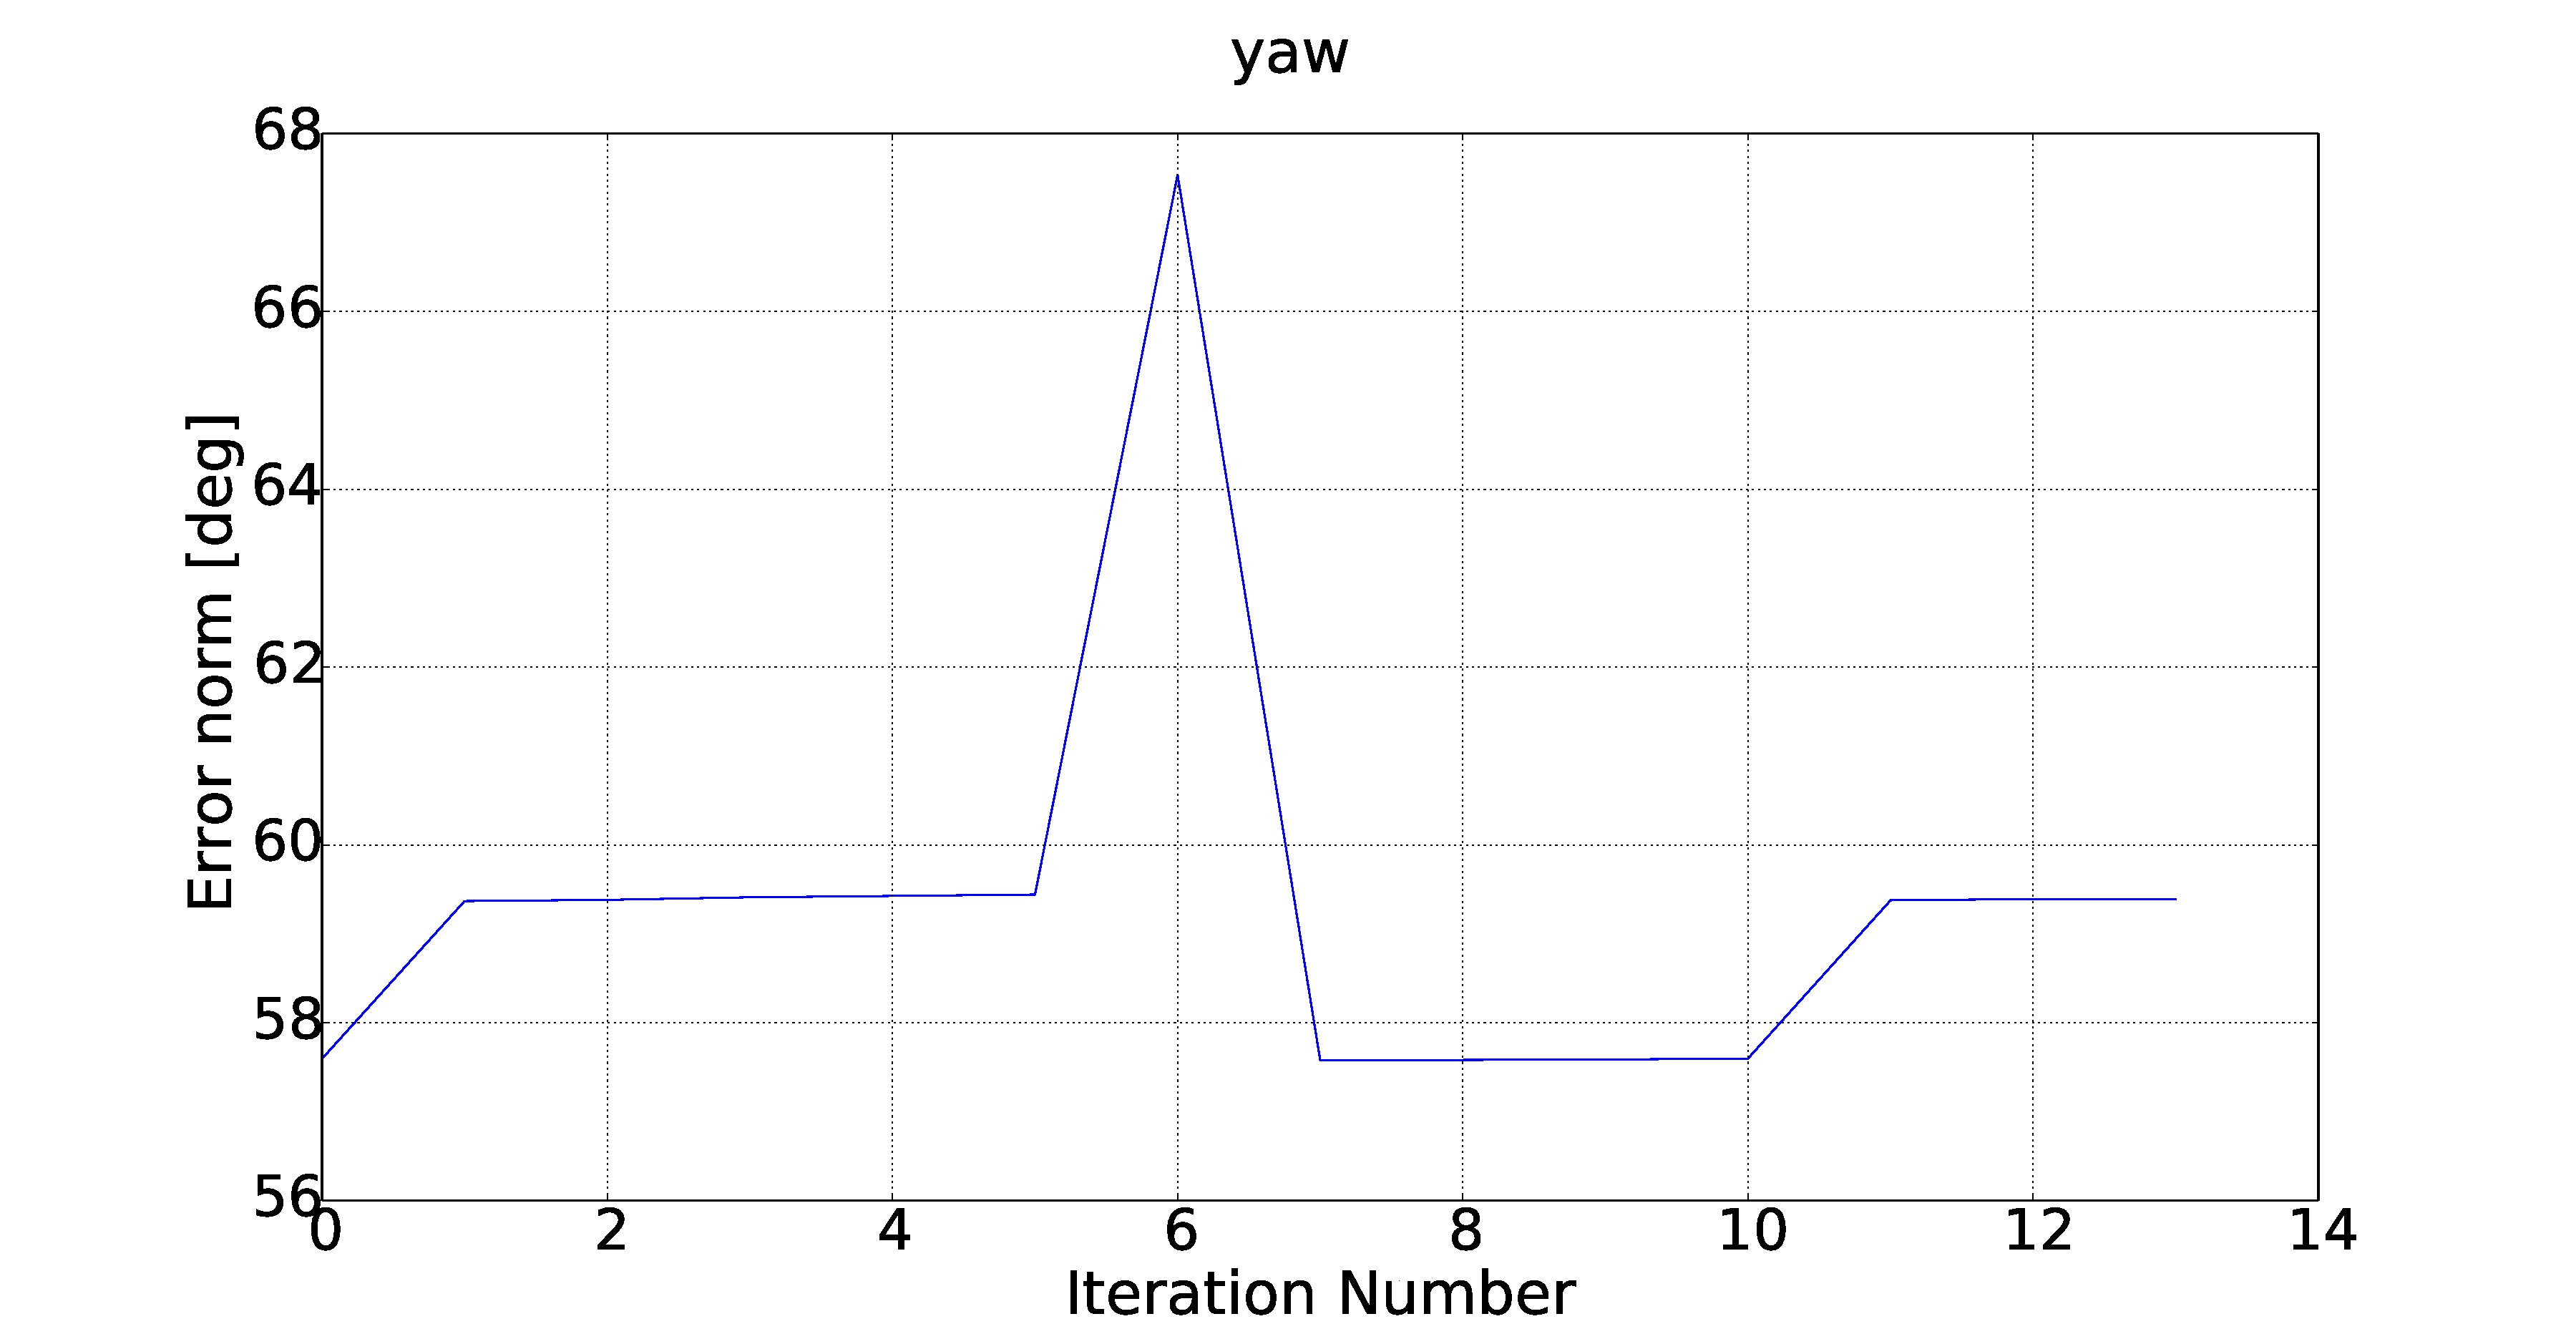
\includegraphics[width=\textwidth]{figures/chapter3/err_yaw.pdf}
    \caption{Error convergence in the $\psi$ dimension [degrees].}
\label{fig:err-convergence-psi}
  \end{subfigure}
  \caption{Plots showing the error in each dimension during for each iteration of the error minimisation procedure.}
  \label{fig:err-convergence}
\end{figure*}

The graphs in Figure~\ref{fig:err-convergence} show that the error gets reduced in the $x$ and $z$ dimensions, while it gets worse in the $y$ and rotation dimensions. Since the optimisation procedure is based on the error in the translation vector, it is not surprising that the rotation error grows. However, the $y$ dimension error growing is somewhat surprising.  %These figures show that the error hovers around 0 after only a few iterations, but does not fully converge. This may warrant some investigation, but it is suspected that the focal length step sizes are too large and must be adapted between iterations. This will be implemented in later versions.

Upon closer inspection, it can be seen that of the three translation vectors, the $y$ dimension has the lowest total error. Since all three vectors carry the same importance weighting for optimisation, it is inevitable that the $x$ and $z$ dimension's errors get lowered at the cost of the $y$ dimension's accuracy. 

\subsection{Test for Normality}
\label{sec:err-norm-test}

To check if $\bm{\epsilon}$ is indeed normally distributed as assumed in Equation~\ref{eq:chap3-eq2-offset}, a frequency histogram of the error matrix $\epsilon$ in all six dimensions are plotted along with a normal distribution drawn using each dimension's mean and standard deviation. A $\chi^2$ test could also have been used. However, it was found that the sample size of the data set was too large and it is known that some skewness in the data can have a large impact on the $\chi^2$ probability estimate CITE???. Therefore, a graphical approach was taken to determining if the errors are normally distributed around 0.0. 

Figure~\ref{fig:err-norm} shows the frequency histogram plots of the CVS measurement errors in the six dimensions. A normal distribution, using the averages and standard deviations from the data set, are superimposed to illustrate the normal distribution of the data.

\begin{figure*}
  \begin{subfigure}{0.45\textwidth}
    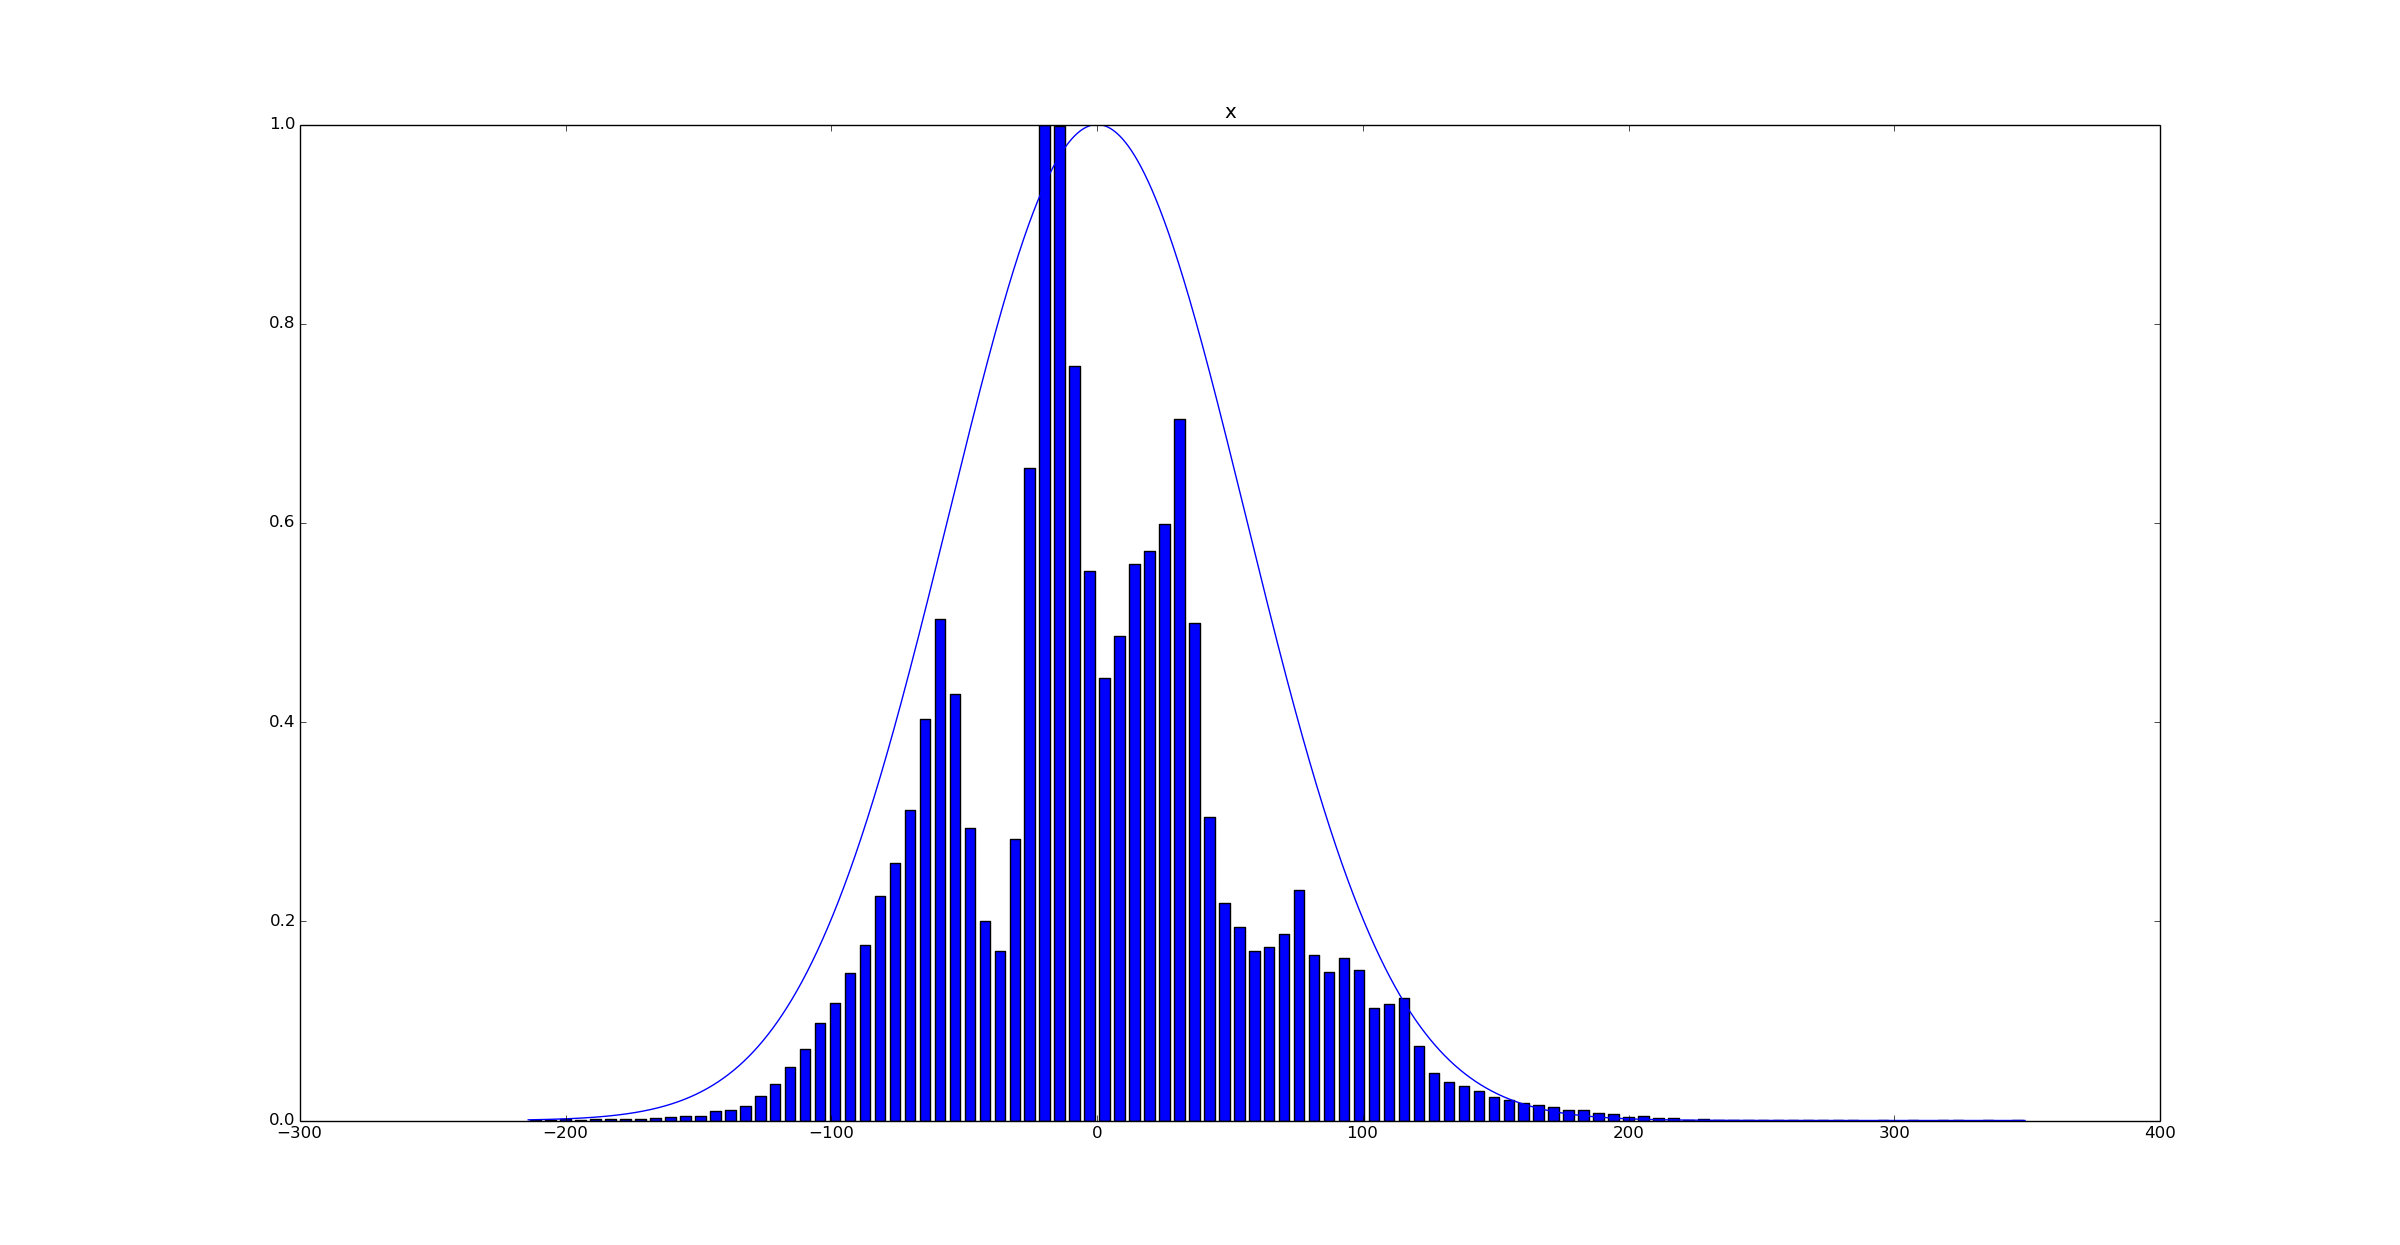
\includegraphics[width=\textwidth]{figures/chapter3/norm_x}
    \caption{Histogram of the error in the $x$ dimension with a mean of $-5.17\mu$mm and a standard deviation of 293mm.}
  \end{subfigure}
~
  \begin{subfigure}{0.45\textwidth}
     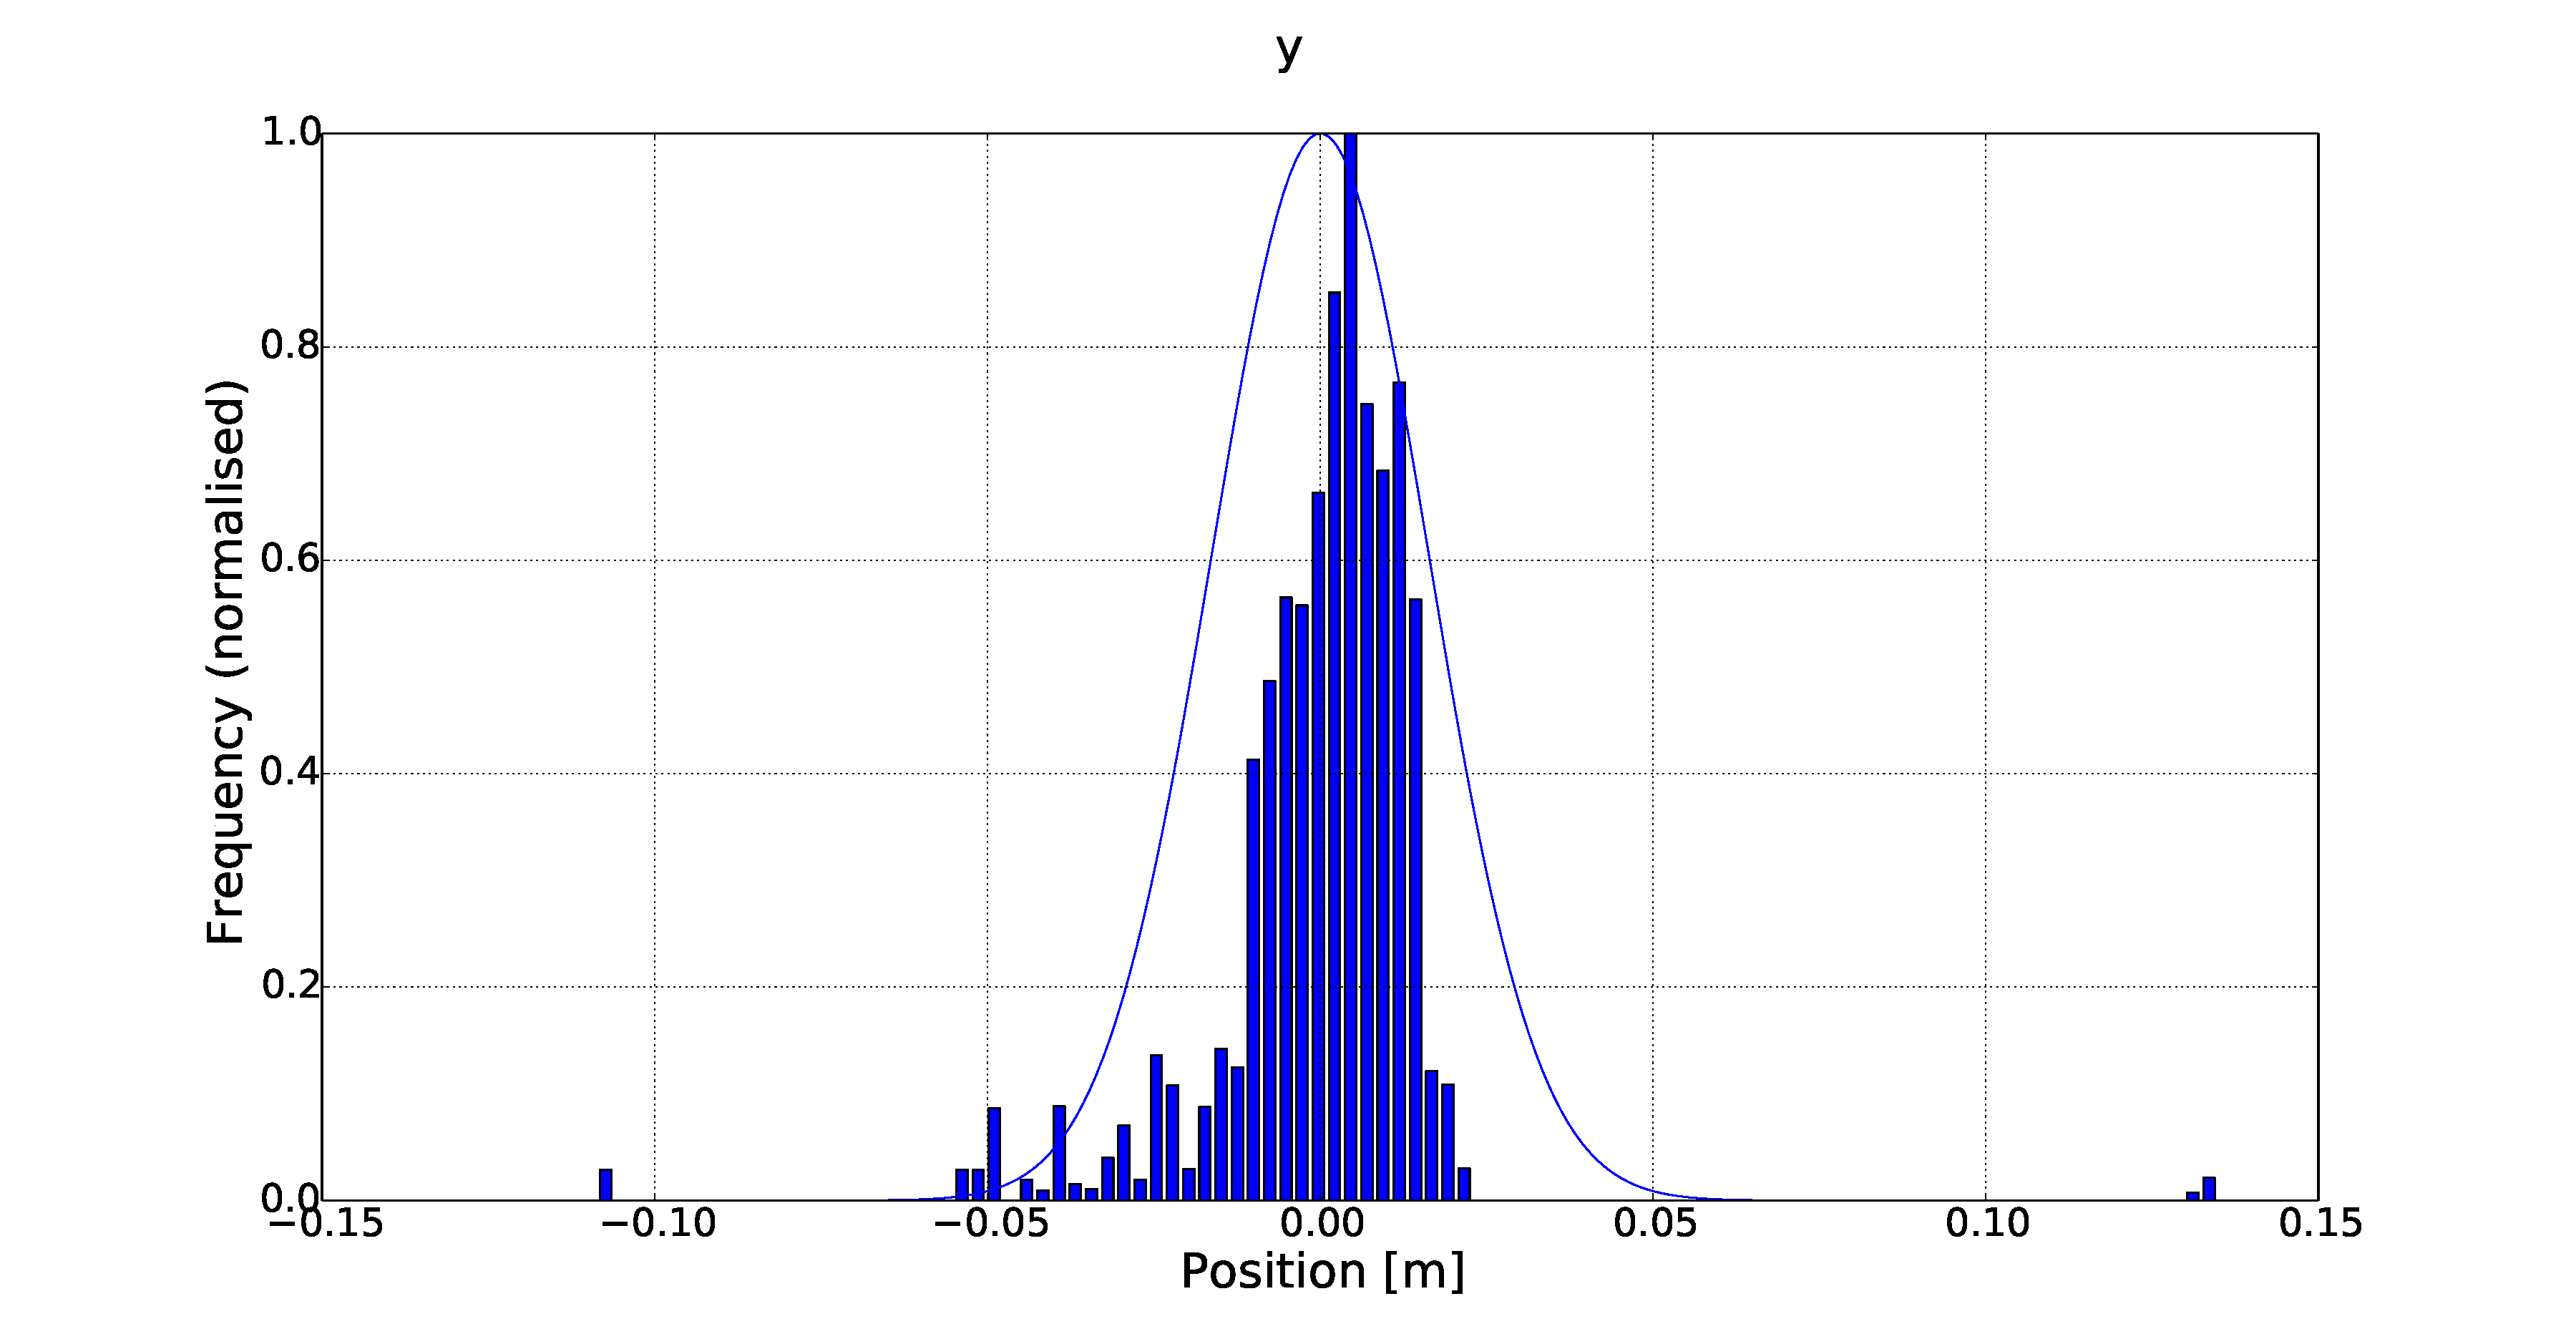
\includegraphics[width=\textwidth]{figures/chapter3/norm_y}
     \caption{Histogram of the error in the $y$ dimension with a mean of $-20.2\mu$mm and a standard deviation of 167mm.}
  \label{fig:norm-y}
  \end{subfigure}
~
  \begin{subfigure}{0.45\textwidth}
     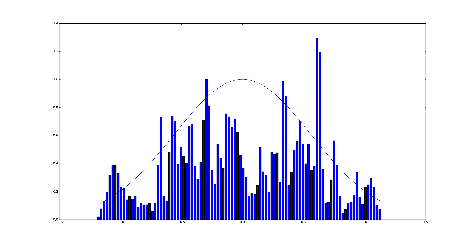
\includegraphics[width=\textwidth]{figures/chapter3/norm_z.pdf}
     \caption{Histogram of the error in the $z$ dimension with a mean of 1.17mm and a standard deviation of 560mm.}
  \label{fig:norm-z}
  \end{subfigure}
~
  \begin{subfigure}{0.45\textwidth}
     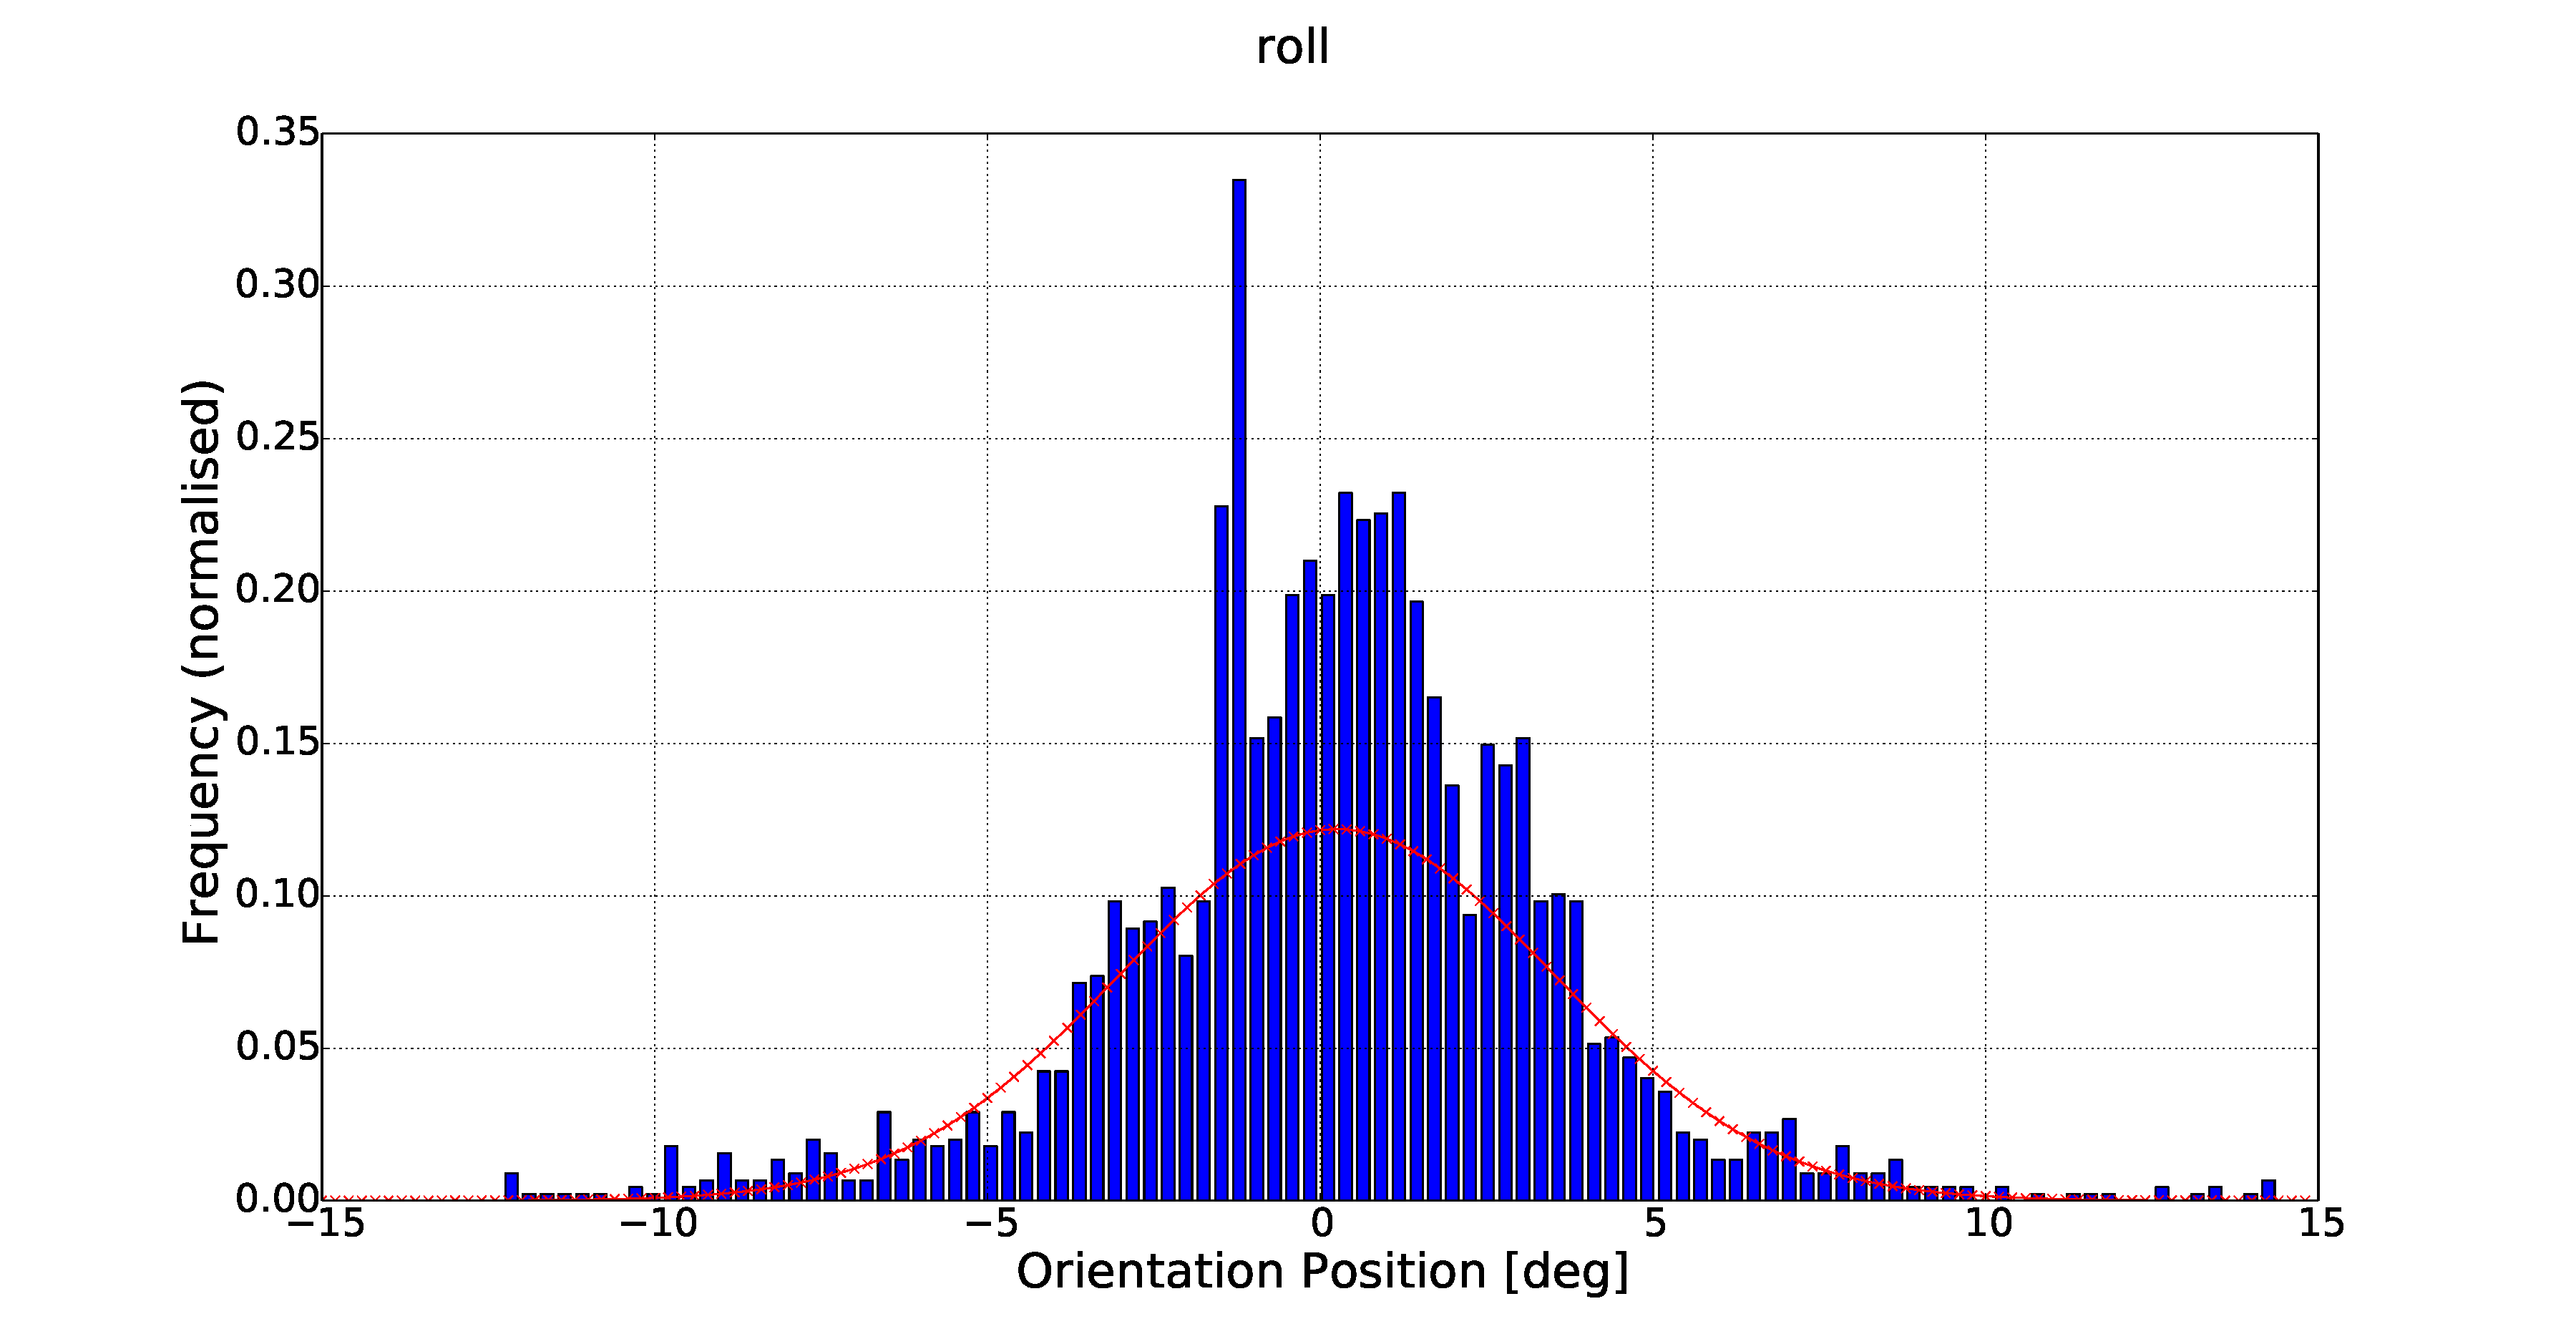
\includegraphics[width=\textwidth]{figures/chapter3/norm_roll.pdf}
     \caption{Histogram of the error in the $\theta$ dimension with a mean of 4 mili-degrees and a standard deviation of 44.0\degree.}
  \label{fig:norm-roll}
  \end{subfigure}
~
  \begin{subfigure}{0.45\textwidth}
     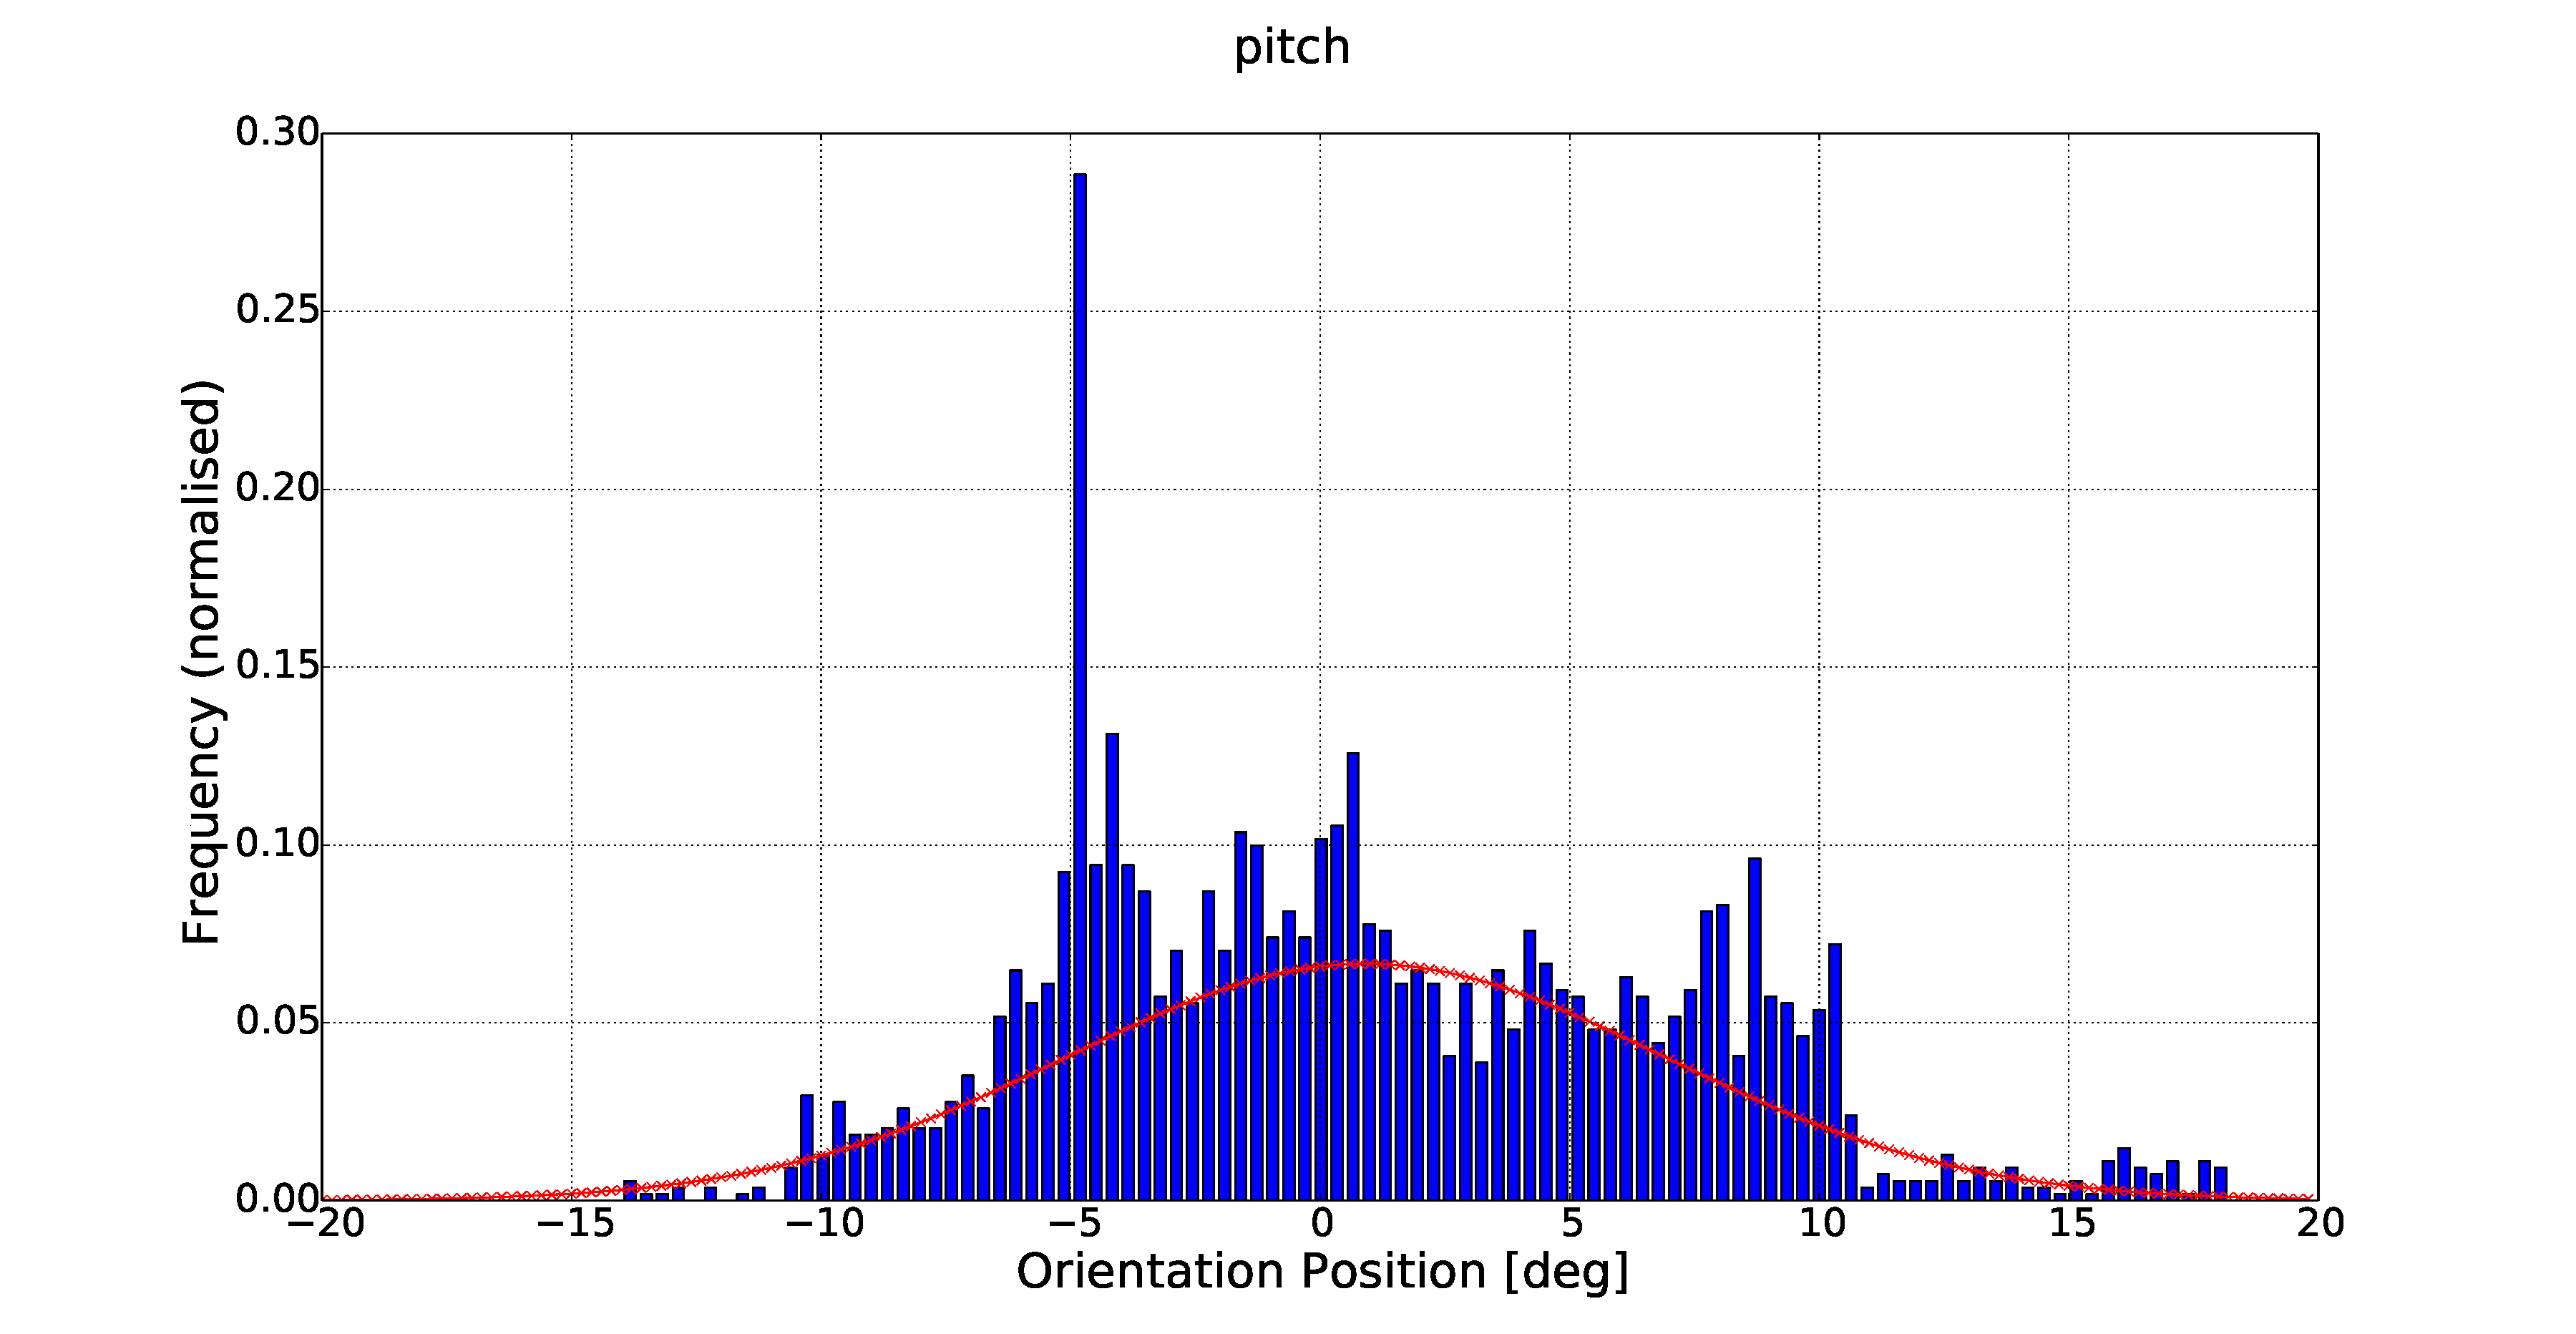
\includegraphics[width=\textwidth]{figures/chapter3/norm_pitch.pdf}
     \caption{emem}
  \label{fig:norm-pitch}
  \end{subfigure}
~
  \begin{subfigure}{0.45\textwidth}
     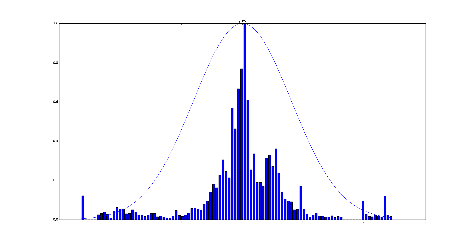
\includegraphics[width=\textwidth]{figures/chapter3/norm_yaw.pdf}
     \caption{memememe}
  \label{fig:norm-yaw}
  \end{subfigure}
  \caption{meme}
  \label{fig:err-norm}
\end{figure*}

It can be seen that all the plots are roughly centred around 0.0 and are very nearly normally distributed, with the $z$ dimension displaying the largest standard deviation of approximately 500mm. Again, a bad depth estimate is to be expected when working with a single camera.

In all, the histogram plotsof the errors show that the assumption made in Equation~\ref{eq:chap3-eq2-offset} that the errors are normally distributed around 0.0, is roughly a valid one. 

\subsection{Optimum Focal Lengths and Offset}

As a result of the focal length and offset optimisation process, the optimal focal lengths, $f_x$ and $f_y$ were found to be 628 and 535 after 50 iterations of the optimisation algorithm, which is considerably less than the optimum of 700 produced by OpenCV's calibration toolbox. Note that these units are given in camera pixel units and not millimetres. The optimal offset $\bar{\bm{P}}$ was found to be approximately

\[
  [240.8mm \; 40.09mm \; 375.9mm \; \ang{184.3} \; \ang{-2.697} \; \ang{-179.9}]^T
\]

The values in $\bar{\bm{P}}$ contain any constant error bias that may have been introduced to the system during testing. The offsets in the $\theta$ and $\psi$ dimensions can be explained by the differing axis orientations of the CVS camera and Vicon systems, reorienting it by approximately $\pm$$\ang{180}$. This indicates that the offset was correctly calculated and is doing what it is supposed to. The large offset in the $z$ dimension is to be expected, since single camera's are known to produce very bad depth estimates. The offset of 240mm in the $x$ dimension is slightly surprising. %However, it may be explained when it is considered that the origin of the chessboard and camera are on opposite sides of each others' $x$-axis when facing each other. The chessboard's origin would be four blocks, or 400mm, away from the camera's along the $x$-axis, making up for the 320mm offset.

All of the above produce an error 2-norm of approximately 0.81 (normalised), compared to the original 1.15 (normalised). Figure~\ref{fig:estimate} shows the results of the Vicon measurements compared to the original and improved CVS measurements in all six dimensions.

\begin{figure*}
  \begin{subfigure}{0.45\textwidth}
    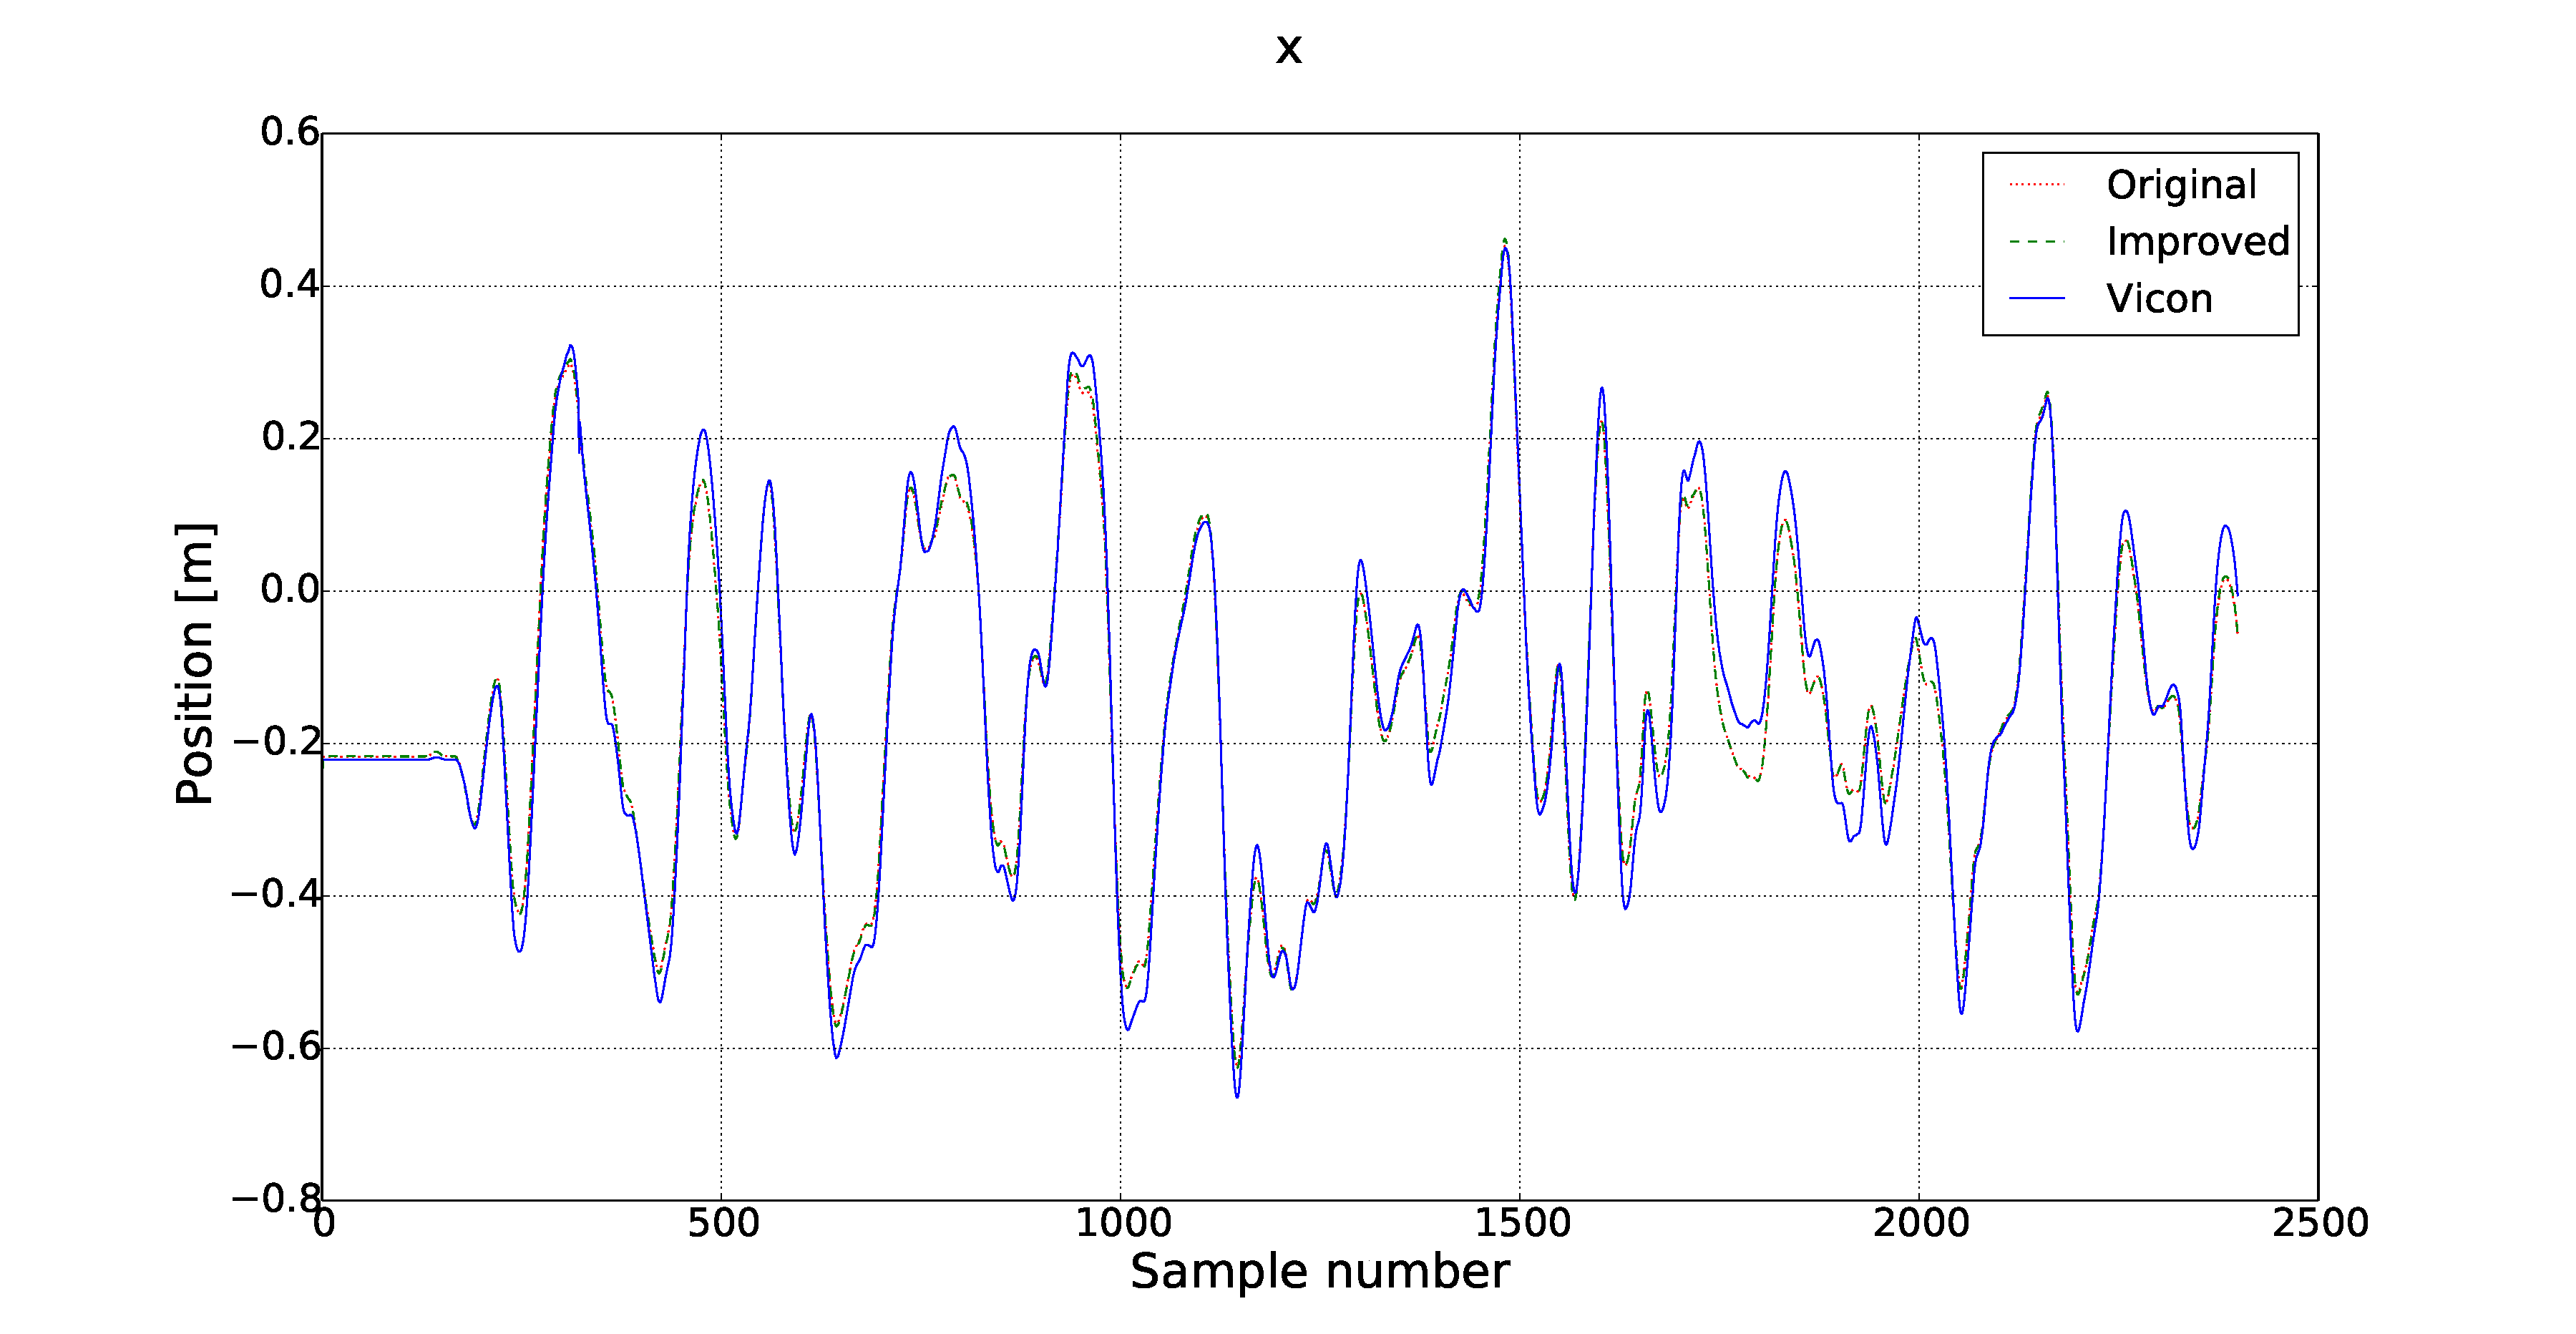
\includegraphics[width=\textwidth]{figures/chapter3/x}
    \caption{The ground-truth Vicon pose estimate, versus the original and improved CV pose estimates in the $x$ dimension.}
  \label{fig:estimate-x}
  \end{subfigure}
~
  \begin{subfigure}{0.45\textwidth}
    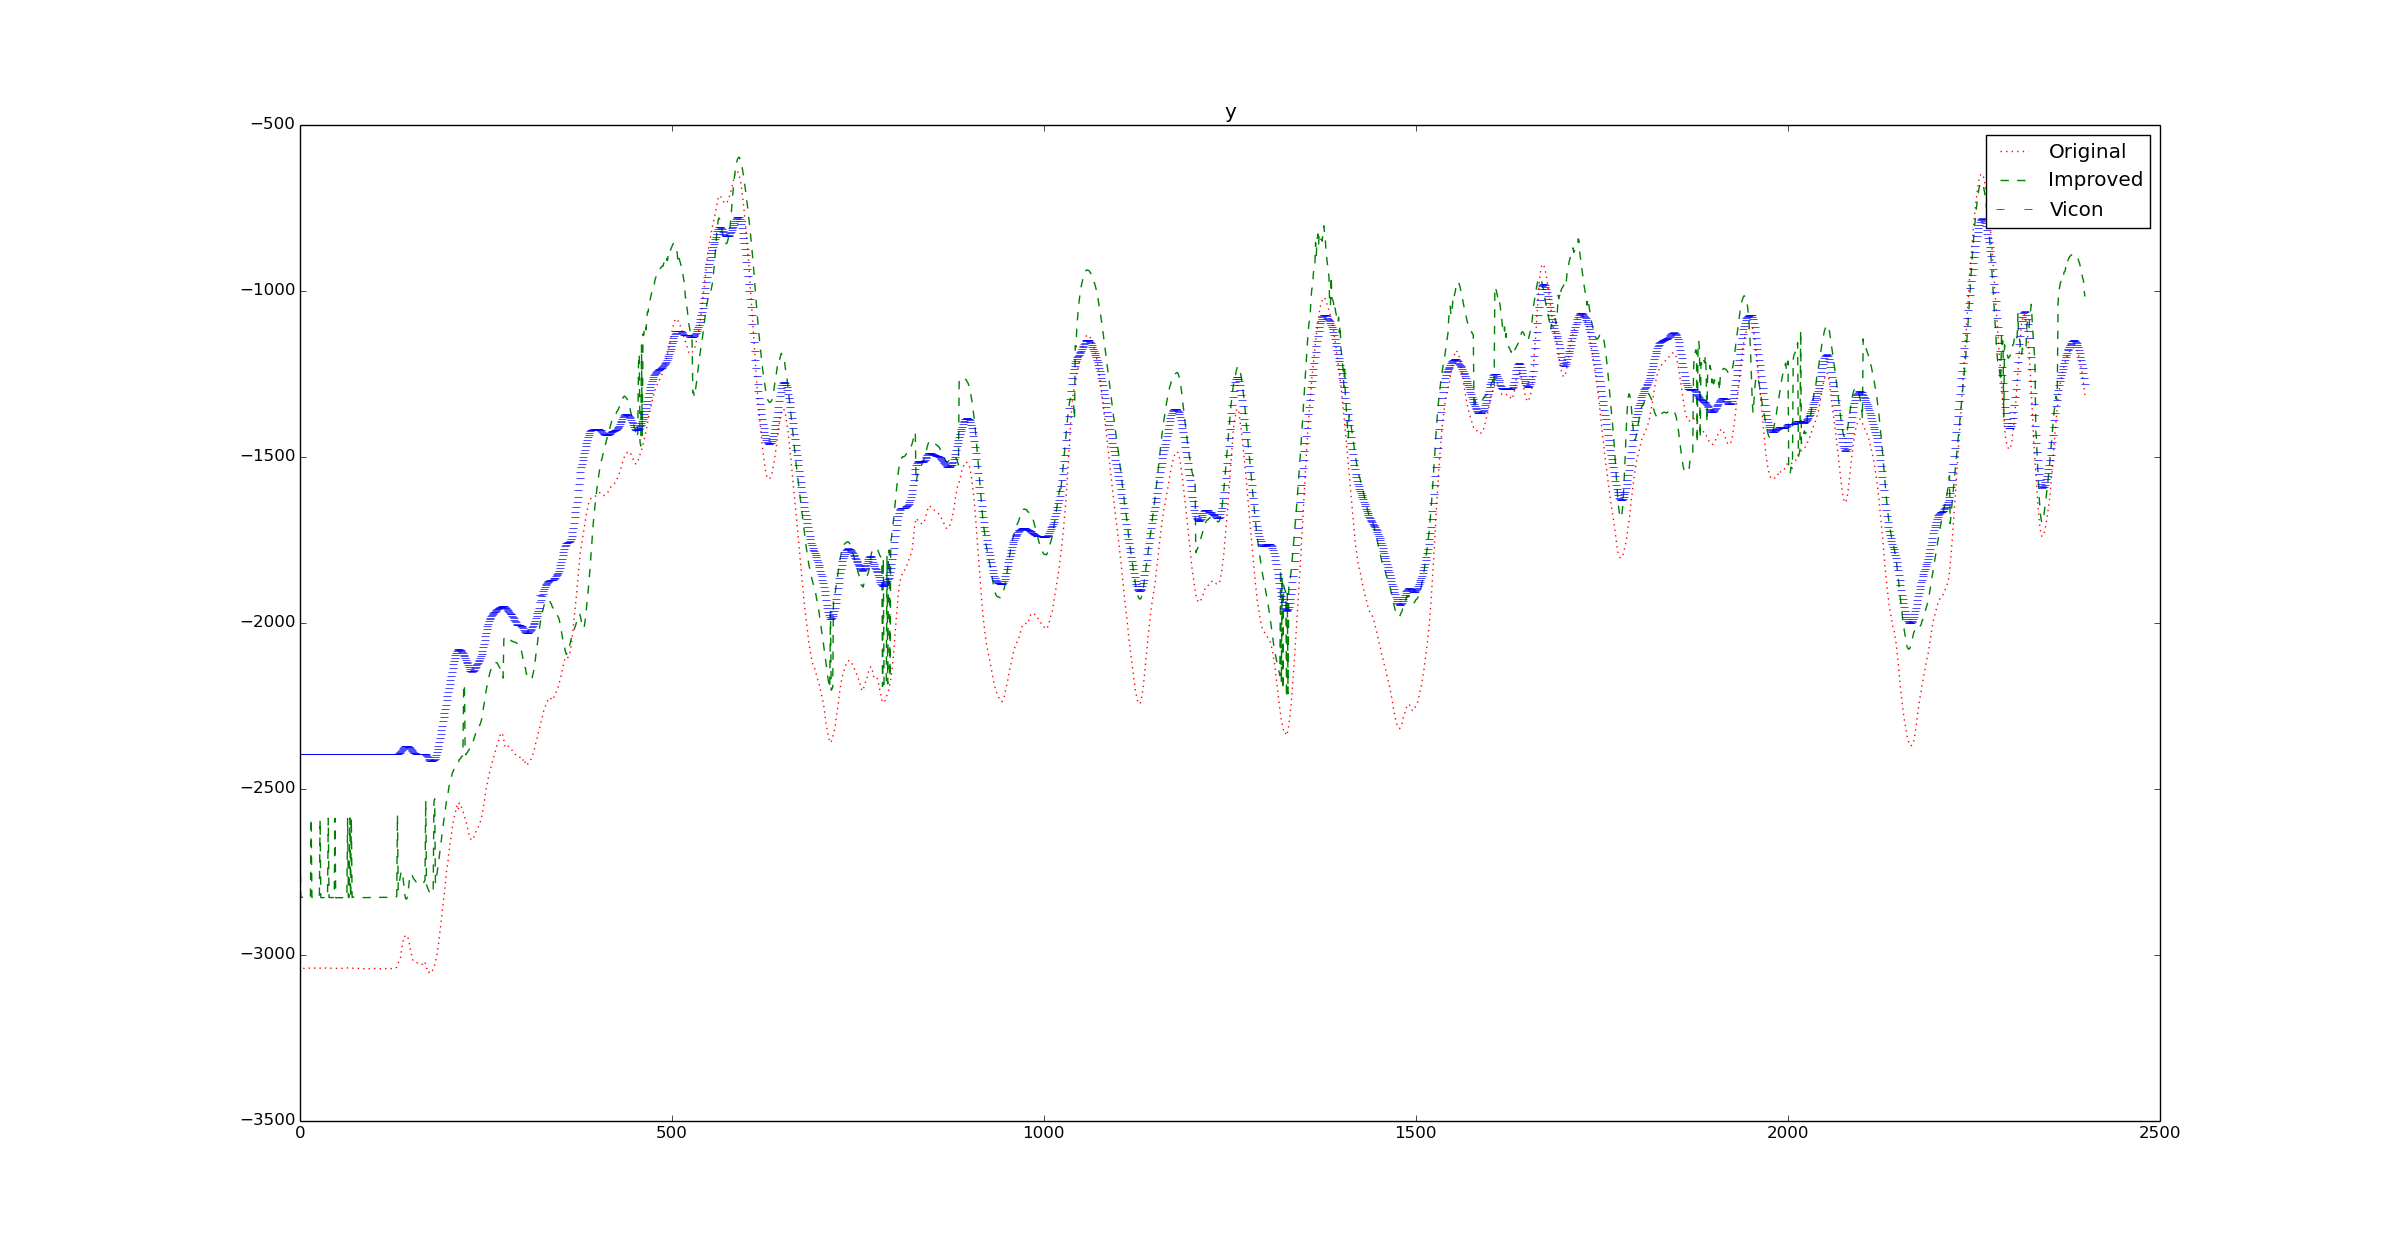
\includegraphics[width=\textwidth]{figures/chapter3/y}
    \caption{The ground-truth Vicon pose estimate, versus the original and improved CV pose estimates in the $y$ dimension.}
  \label{fig:estimate-y}
  \end{subfigure}
~
  \begin{subfigure}{0.45\textwidth}
    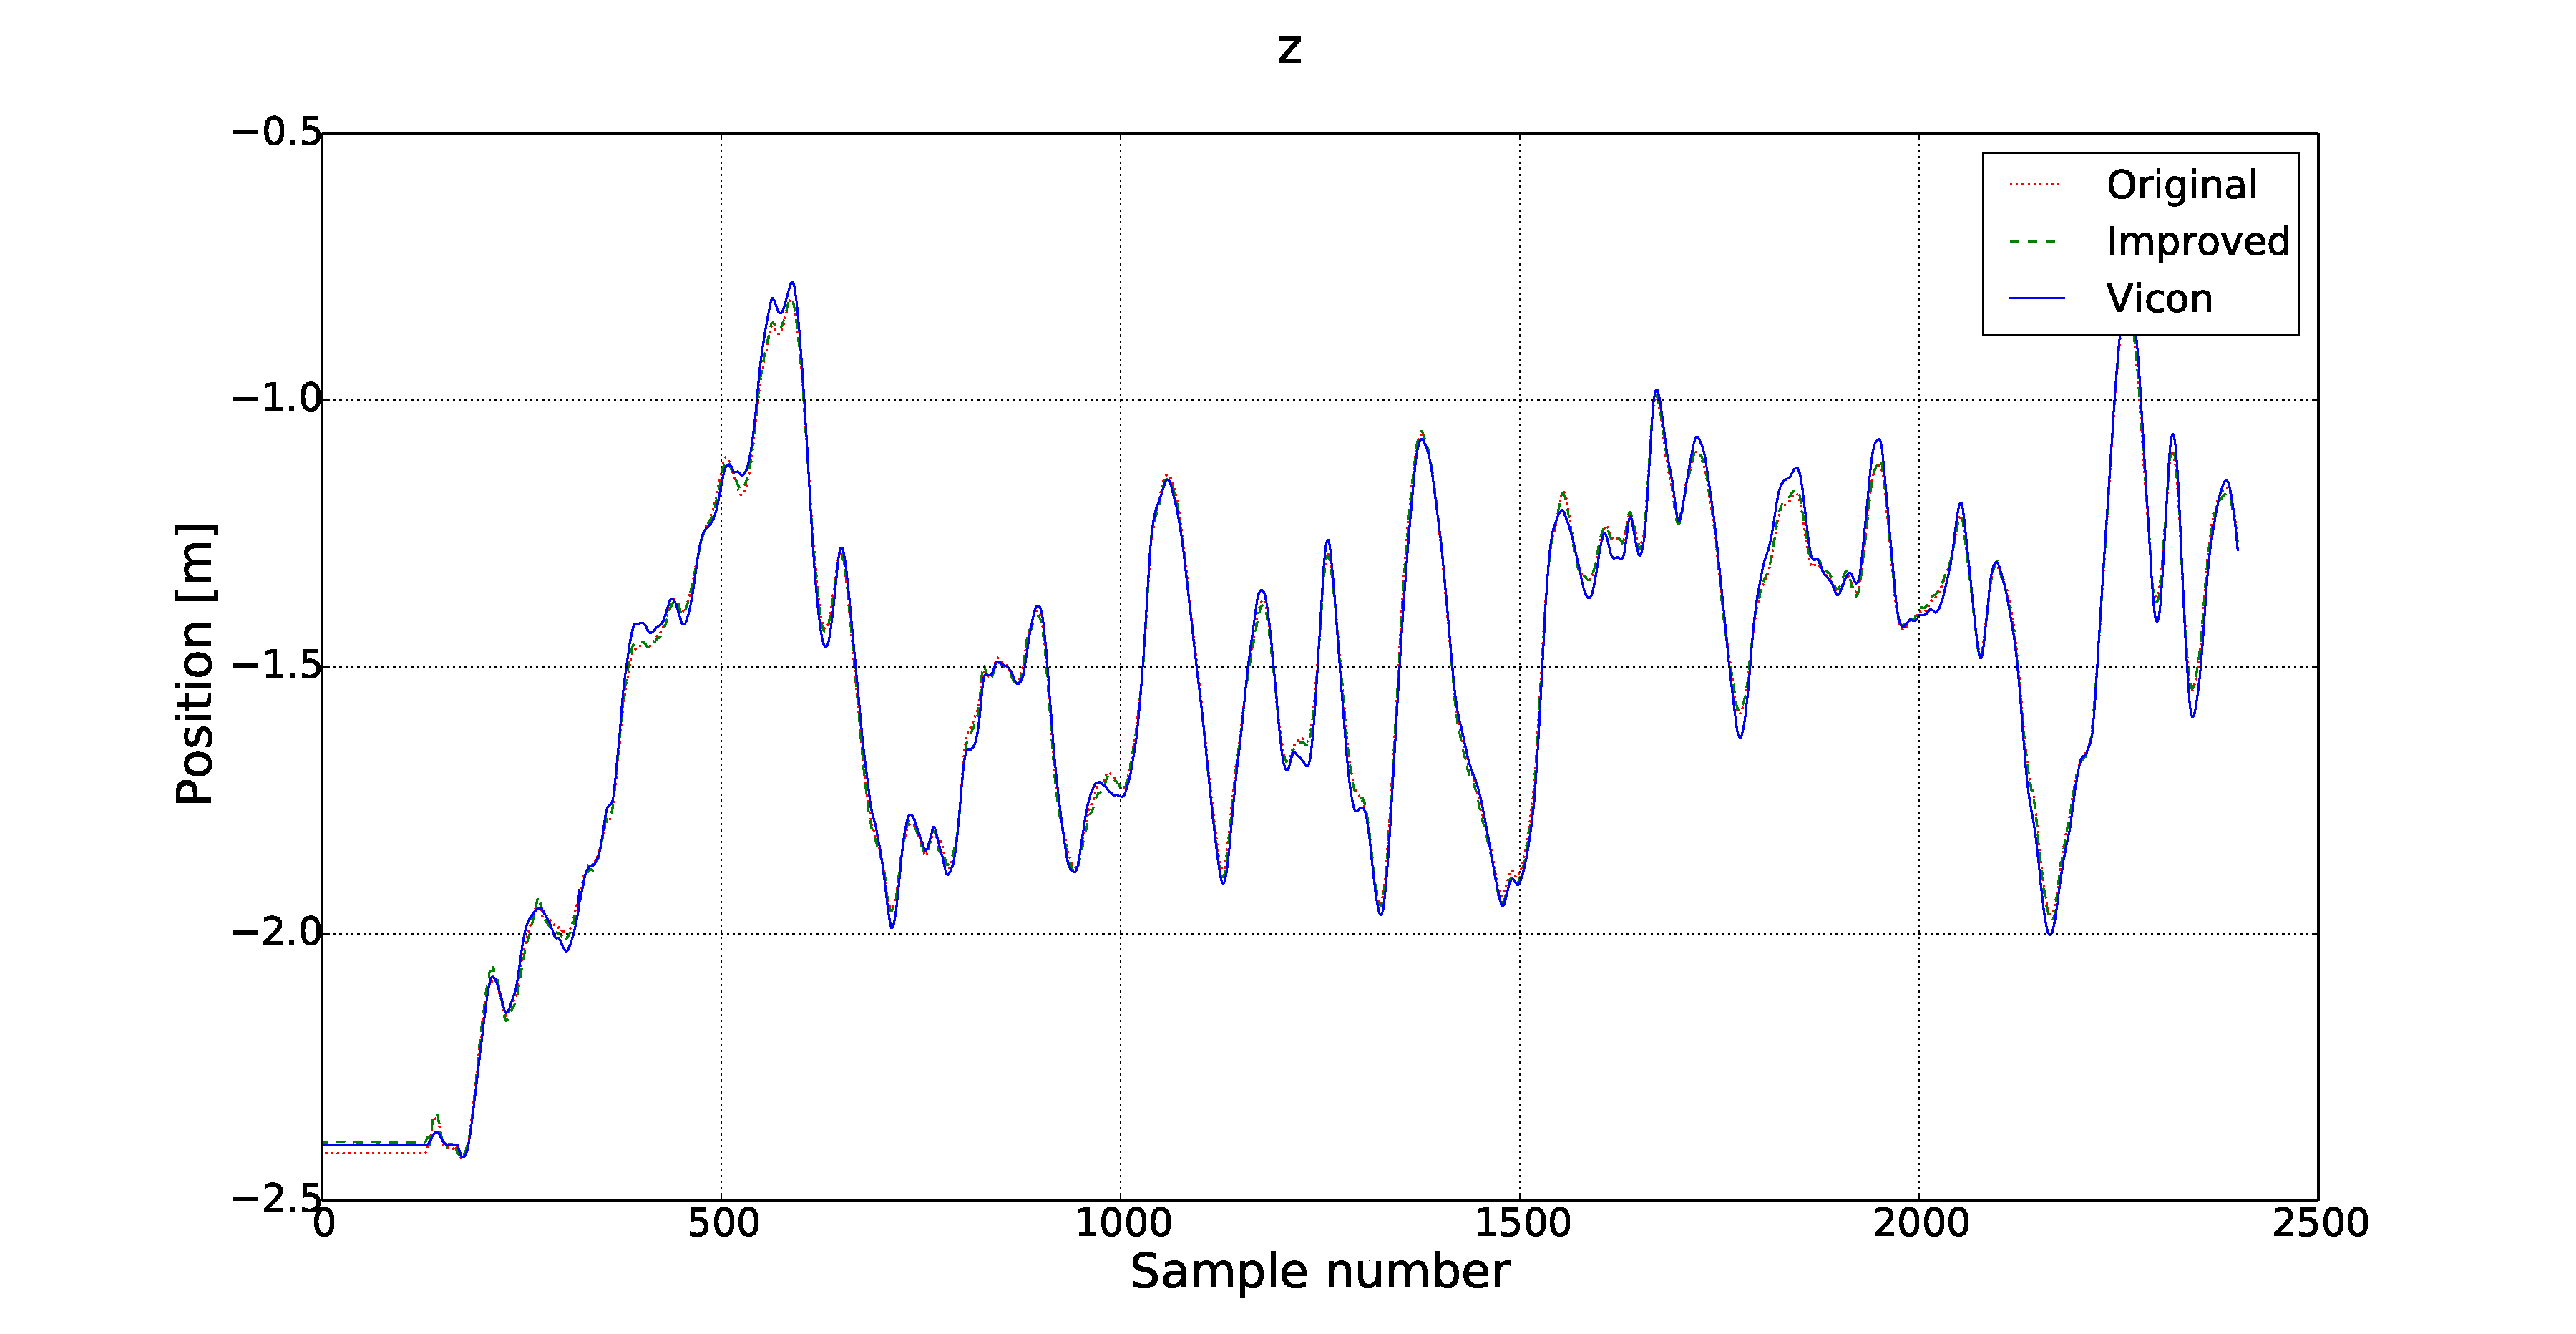
\includegraphics[width=\textwidth]{figures/chapter3/z}
    \caption{The ground-truth Vicon pose estimate, versus the original and improved CV pose estimates in the $z$ dimension.}
  \label{fig:estimate-z}
  \end{subfigure}
~
  \begin{subfigure}{0.45\textwidth}
    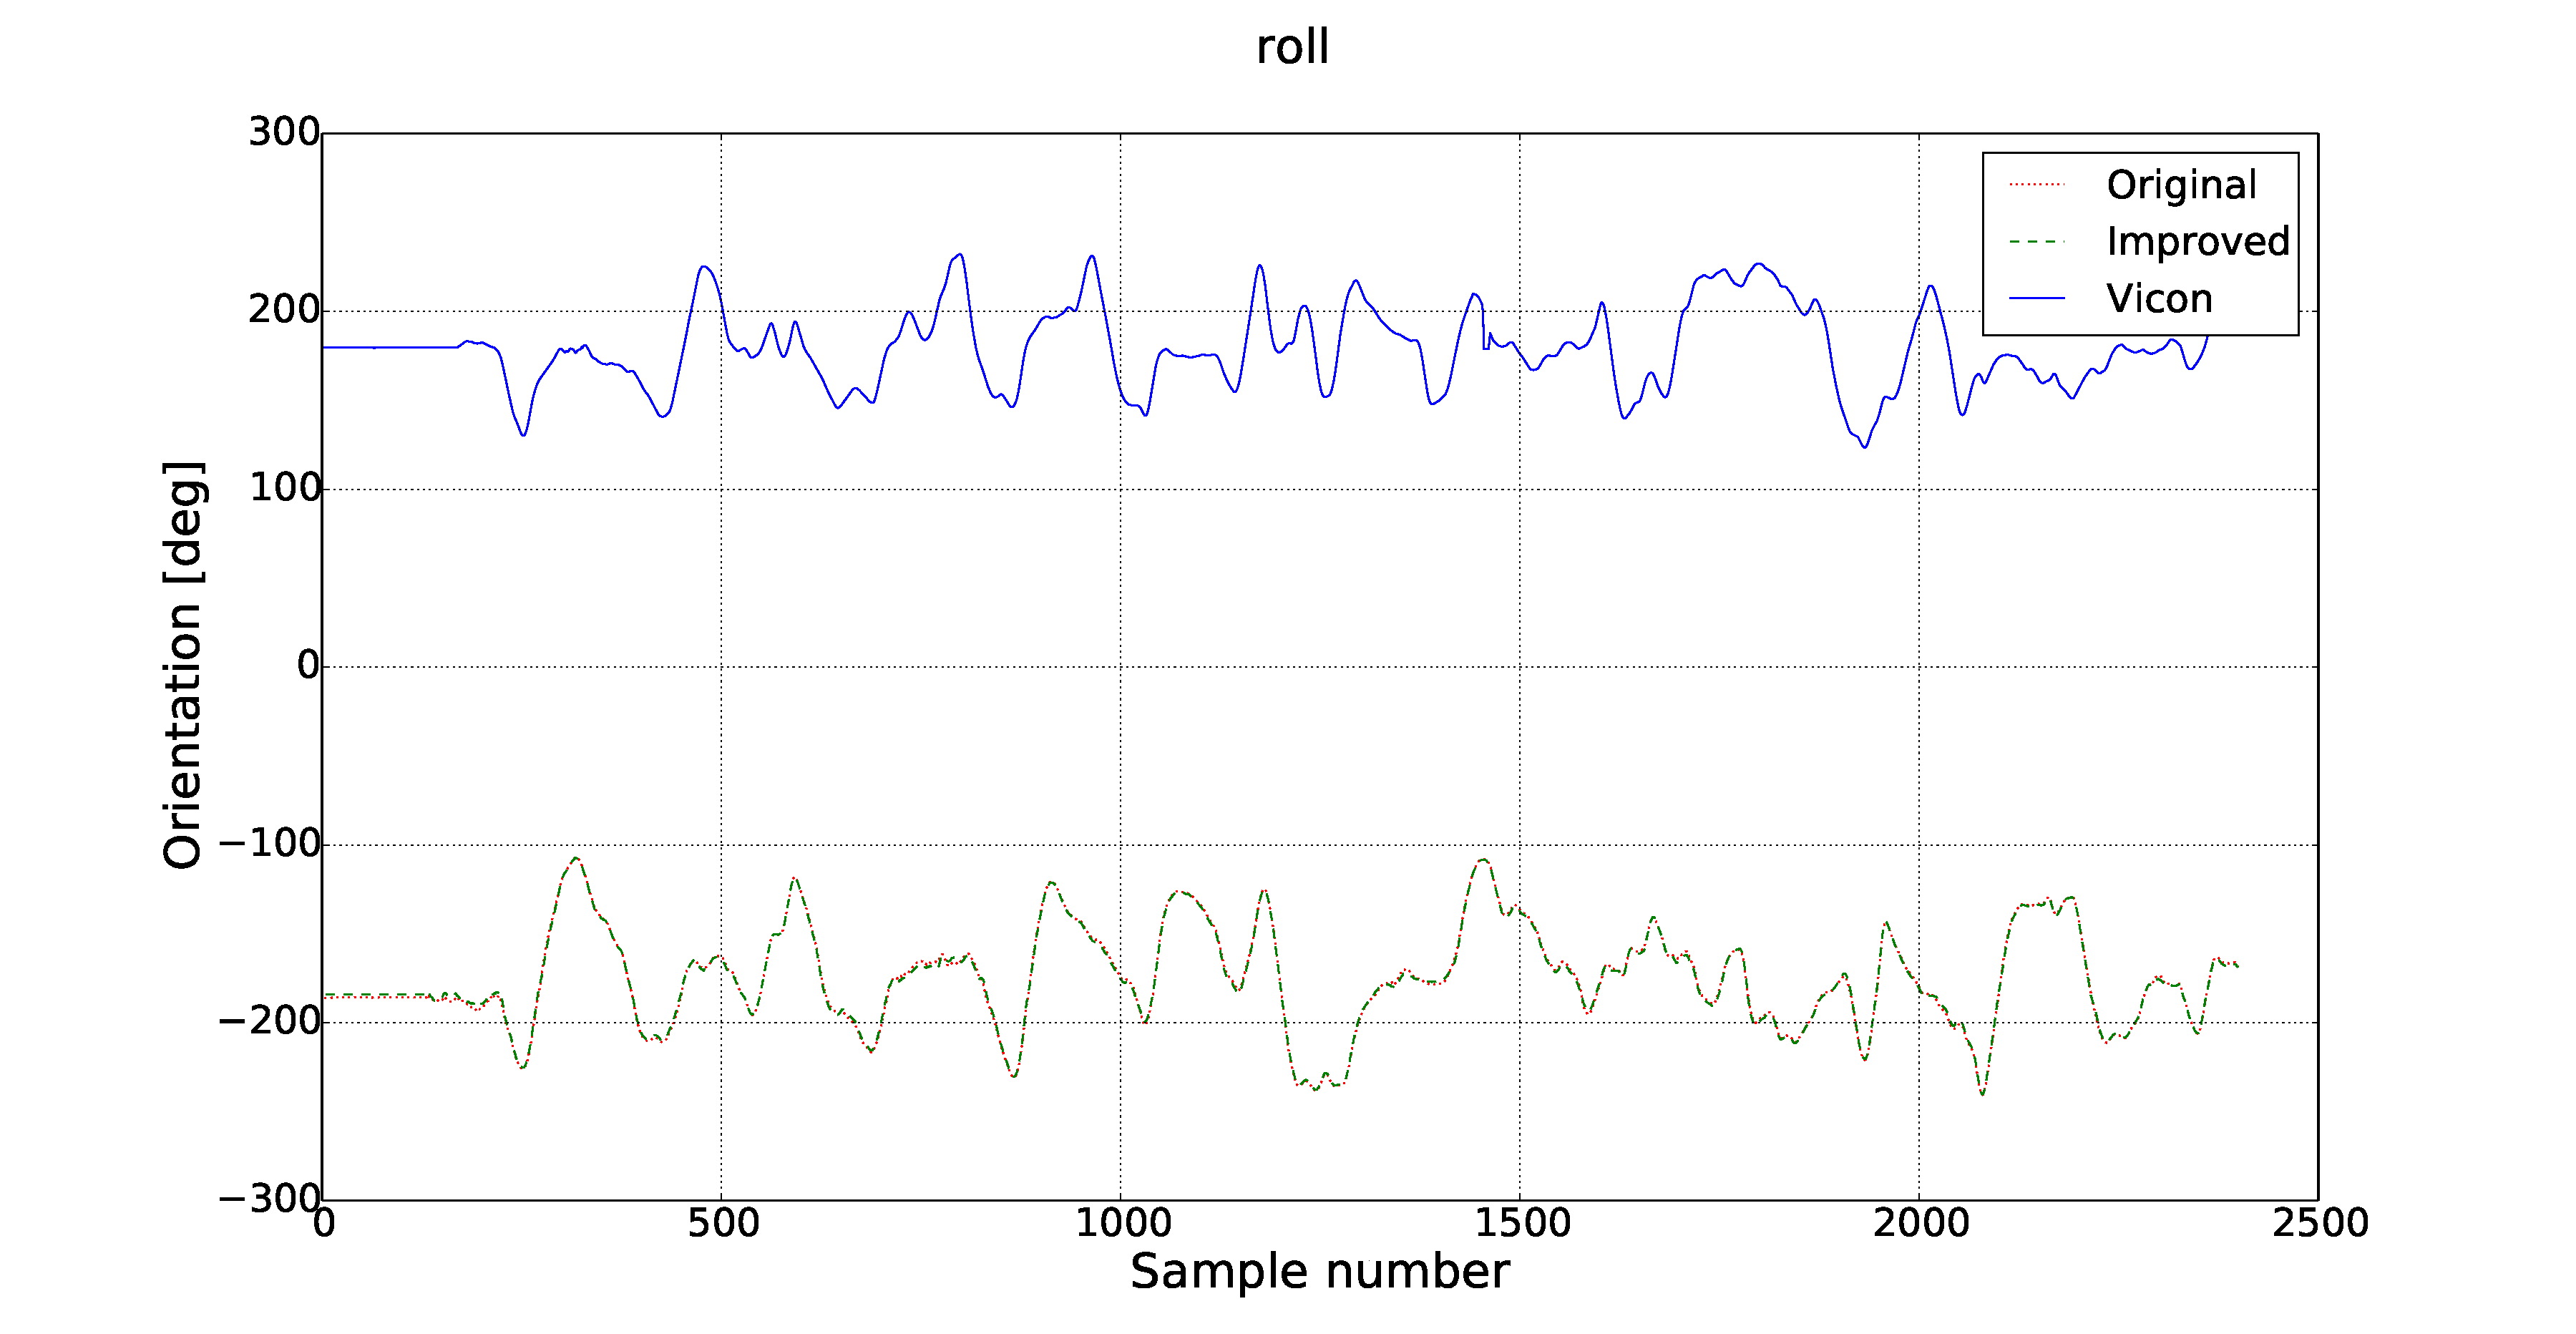
\includegraphics[width=\textwidth]{figures/chapter3/roll}
    \caption{The ground-truth Vicon pose estimate, versus the original and improved CV pose estimates in the $\theta$ dimension.}
  \label{fig:estimate-roll}
  \end{subfigure}
~
  \begin{subfigure}{0.45\textwidth}
    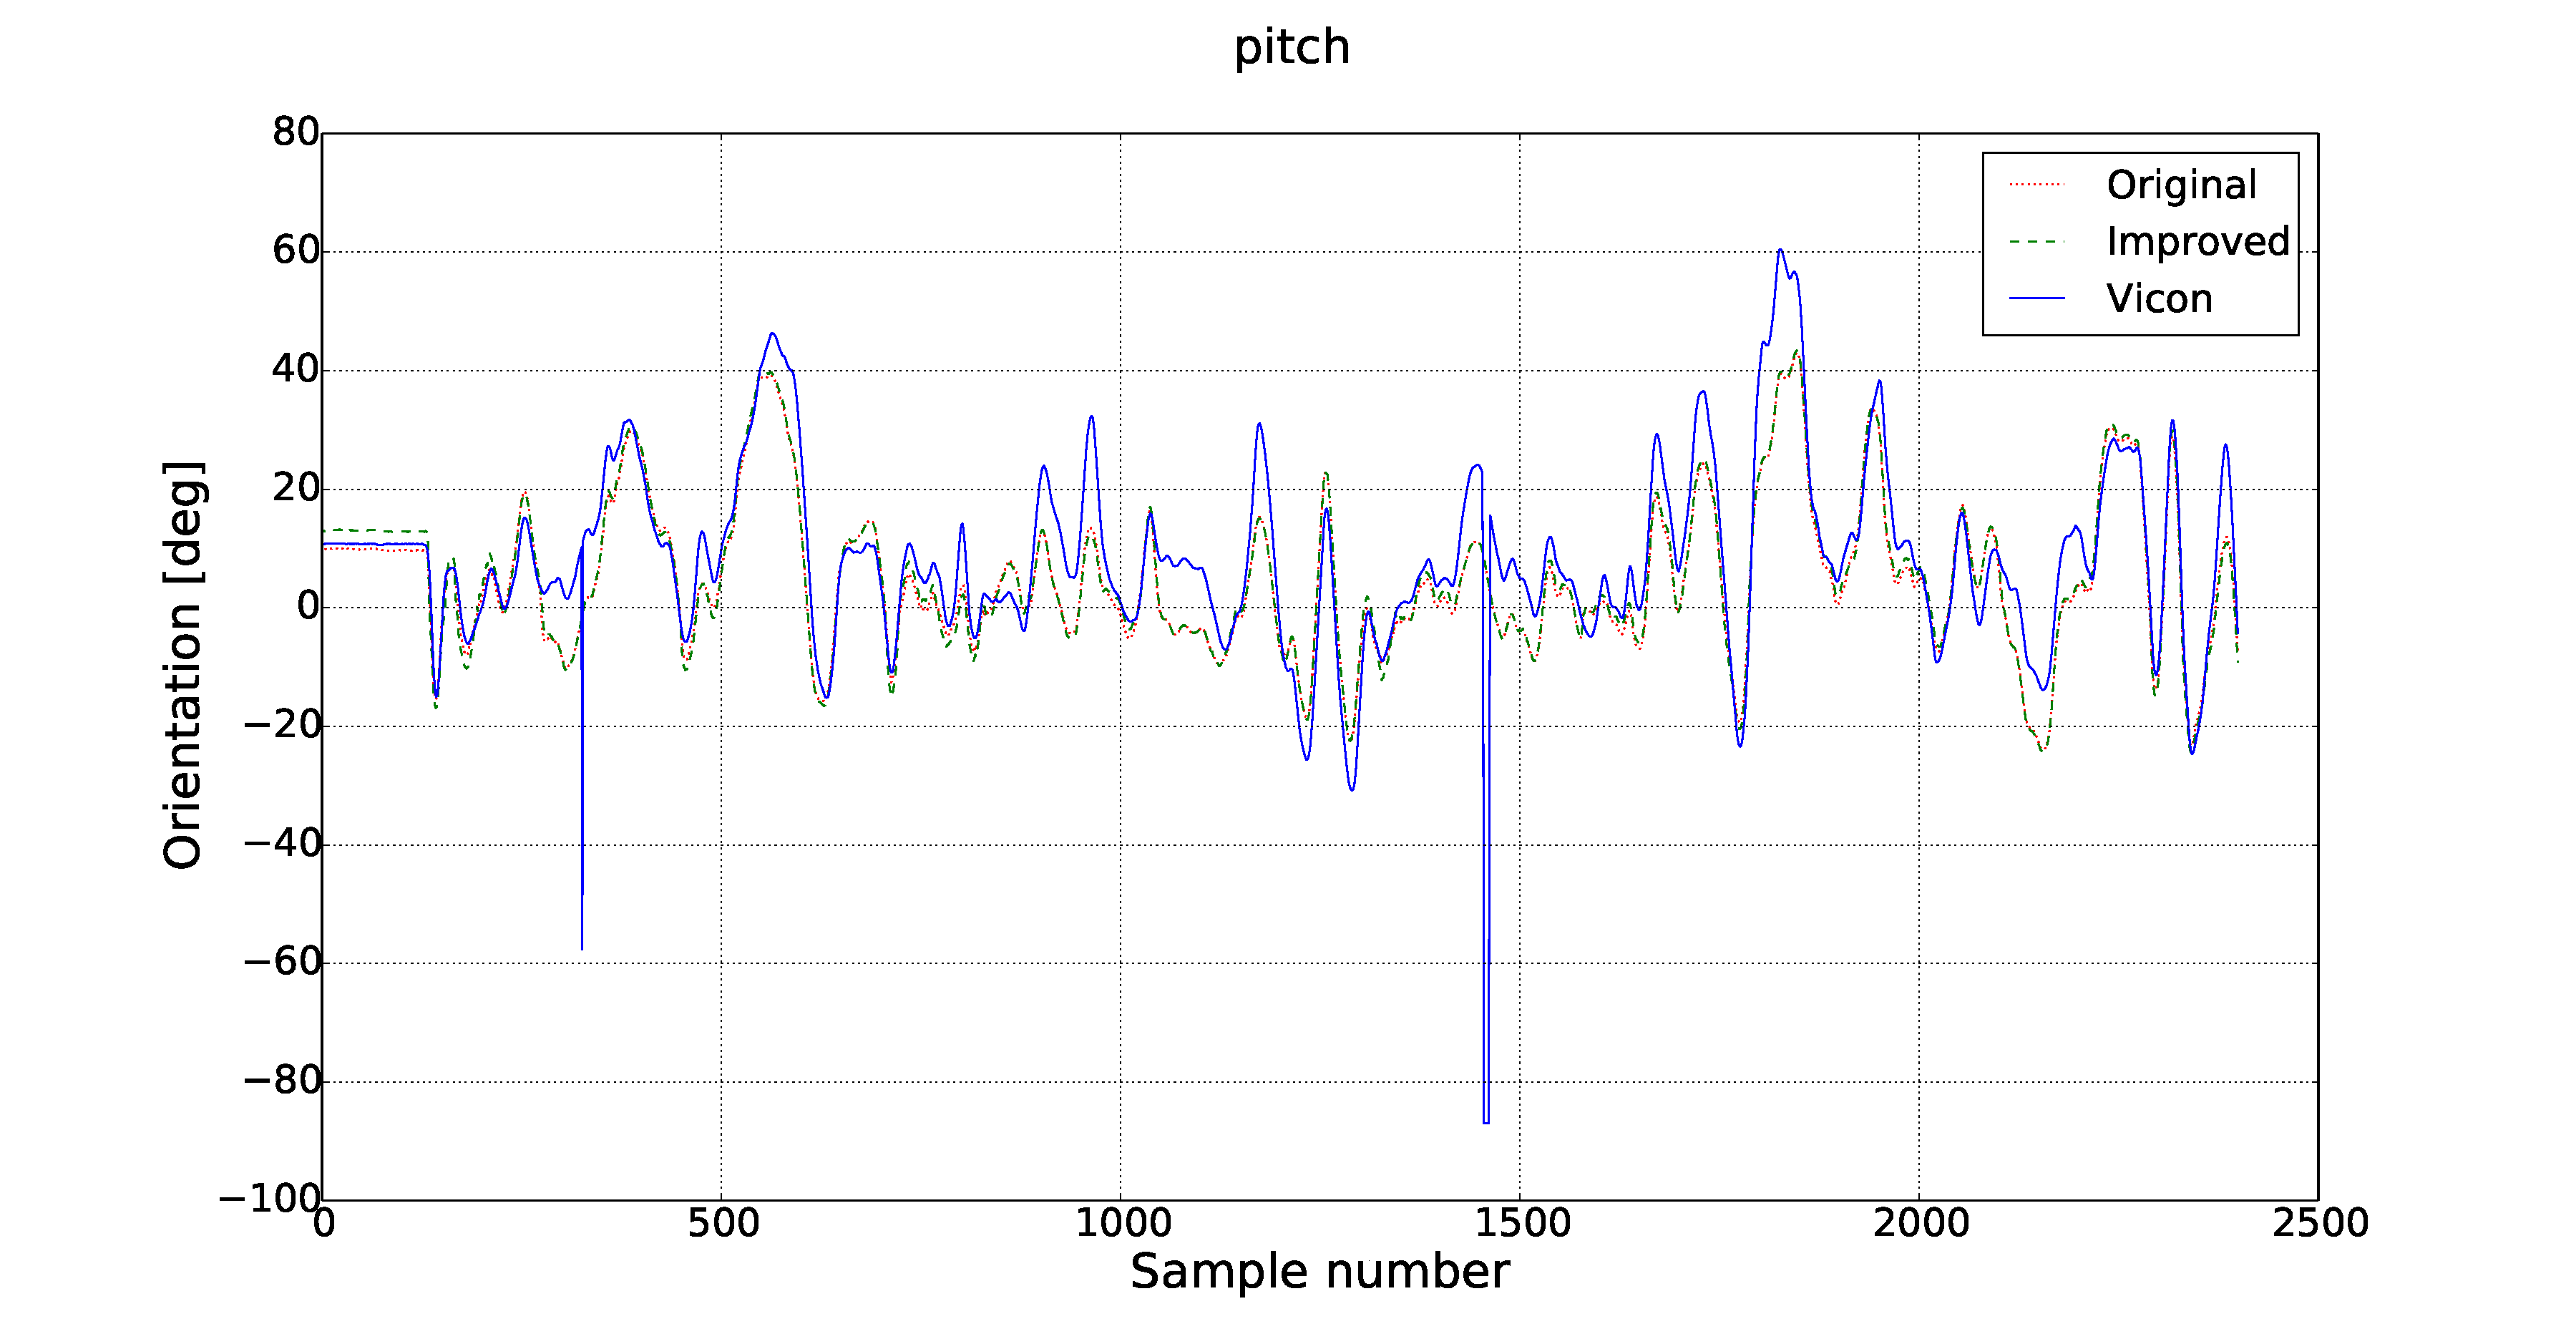
\includegraphics[width=\textwidth]{figures/chapter3/pitch}
    \caption{The ground-truth Vicon pose estimate, versus the original and improved CV pose estimates in the $\phi$ dimension.}
  \label{fig:estimate-pitch}
  \end{subfigure}
~
  \begin{subfigure}{0.45\textwidth}
    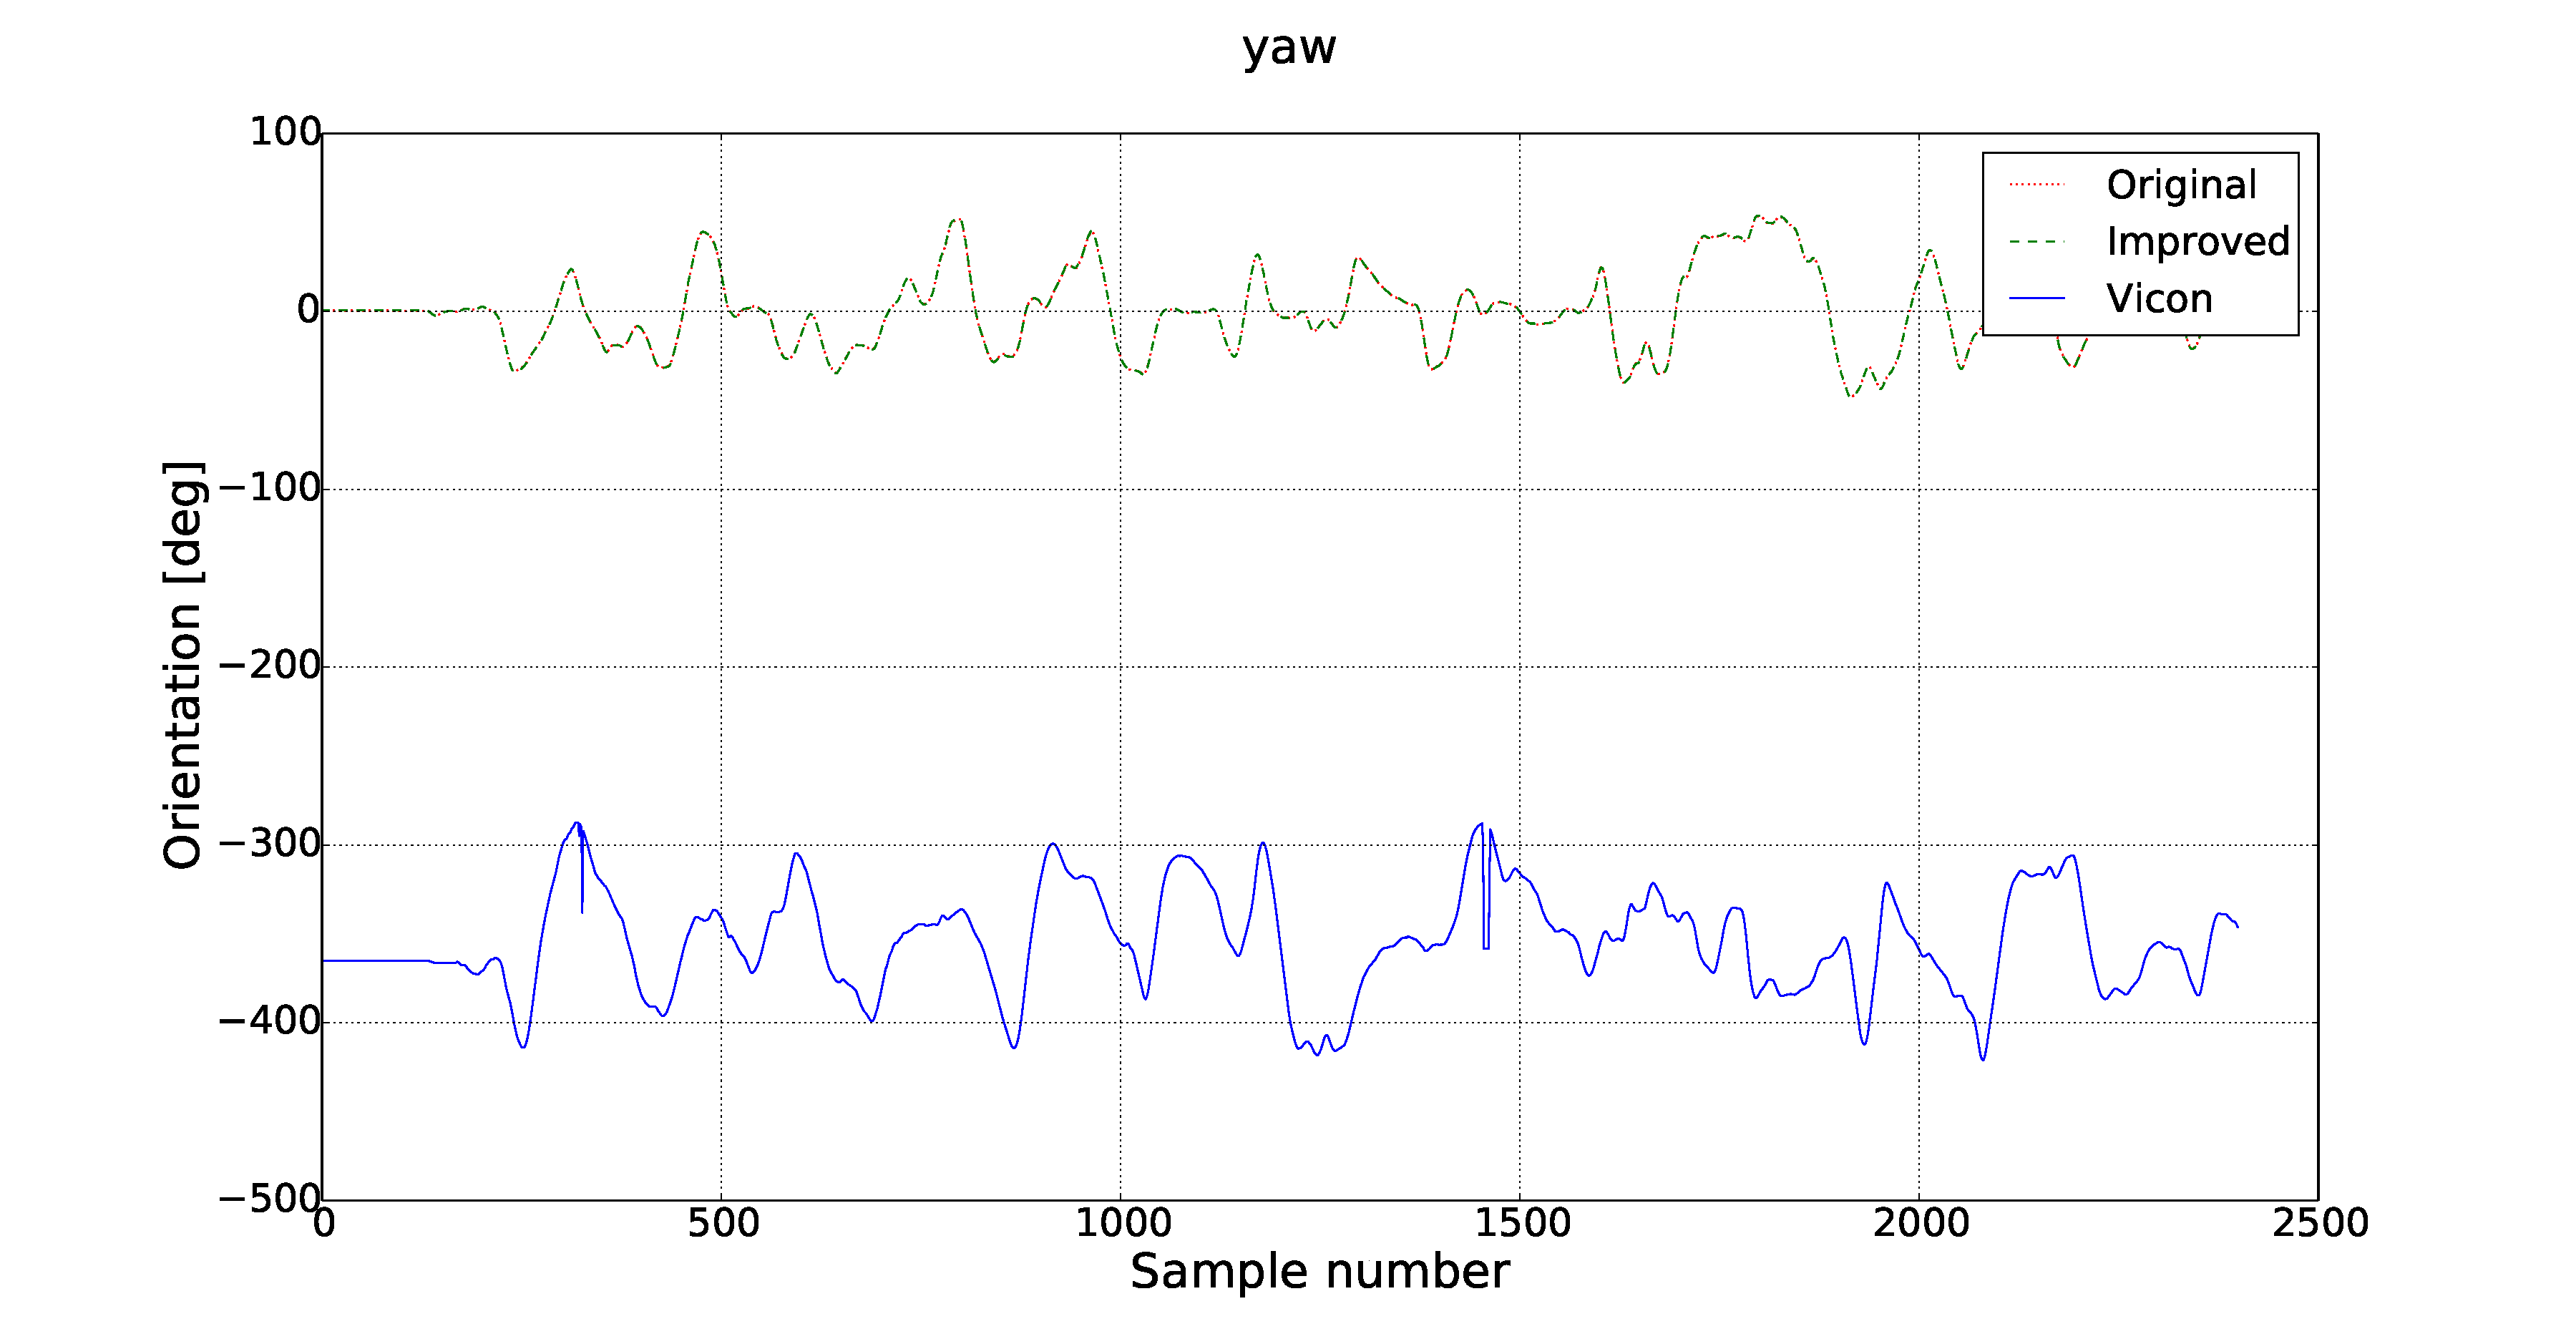
\includegraphics[width=\textwidth]{figures/chapter3/yaw}
    \caption{The ground-truth Vicon pose estimate, versus the original and improved CV pose estimates in the $\psi$ dimension.}
  \label{fig:estimate-yaw}
  \end{subfigure}
  \caption{hello}
  \label{fig:estimate}
\end{figure*}

It can be seen that there is a some improvement in all the dimensions. However, in some cases the improvement is negated by worse results in another place in the data set. This is a result of the optimisation process where an improvement at timeframe $t_i$ in the $x$ dimension, for example, may lead to a worse estimate at time $t_i$ in the $\phi$ dimension. Since the norm of $\bm{\epsilon}$ converges, it can be taken that the improved results are indeed better as a whole, even though it may look like it has gotten worse in the individual dimensions.

\subsection{System Accuracy}

Determining the accuracy of a multi-dimensional model is often a complex task, but the fact that the error is normally distributed makes it possible to use the covariance matrix to check the interdimensional variance and dependence. If it is found that the diagonal of the covariance matrix is sufficiently large relative to the off-diagonal elements, the dimensions can be taken as strongly enough independent of one another and the variance along the diagonal can be taken as a measure of the accuracy. 

The covariance matrix, $\bm{\Sigma}$, was found to be 

\[
  \bm{\Sigma} = 
  \begin{bmatrix}
    \bm{3131.7} & 2255.2 & 98.227 & 94.371 &  98.830 & 106.85 \\ 
    2255.2 & \bm{40924}  & 4038.2 & 197.46 &  30.631 & 1953.7 \\
    98.227 & 4038.2 & \bm{5592.5} & 241.75 &  106.86 & 385.23 \\
    94.371 & 197.46 & 241.75 & \bm{84.939} &  10.303 & 13.792 \\
    98.830 & 30.631 & 106.86 & 10.303 &  \bm{110.54} & 63.381 \\
    106.85 & 1953.7 & 385.23 & 13.792 &  63.381 & \bm{318.17} \\
  \end{bmatrix}
\]

The matrix $\bm{\Sigma}$ shows that there are large off-diagonal elements, indicating that there is strong interdimensional dependence. This unfortunately means that there is no clear indication on the accuracy of the system. However, a probability density function (PDF) can be set up using $\bm{\Sigma}$ that will show what the expected error in the 6 dimensions will be for a given pose. The PDF is given by Equation~\ref{eq:pdf}.

\begin{equation}
  \label{eq:pdf}
  p(\bm{\epsilon}) = \frac{1}{\sqrt{{(2\pi)}^k\lvert\bm{\Sigma}\rvert}}e^{-\frac{1}{2}{(\bm{\epsilon} - \bm{\mu})}^T\bm{\Sigma}^{-1}(\bm{\epsilon} - \bm{\mu})}
\end{equation}

Armed with a PDF and covariance matrix, it is now possible to determine whether the CV system is more accurate than the on-board sensor suite of a drone. 

\section{Conclusion}

